\documentclass[12pt]{article}
\usepackage[utf8]{inputenc}
%\usepackage{nips_2017}
\usepackage{graphicx}
\usepackage{natbib}
\usepackage{booktabs}
\usepackage{float}
\usepackage{amsmath}
\usepackage{psfrag}
\usepackage{epsf}
\usepackage{enumerate}

%\bibliographystyle{apalike}

%\bibliographystyle{unsrt} % Use for unsorted references 
\newcommand{\blind}{0}

%\bibliographystyle{plainnat} % use this to have URLs listed in References

% DON'T change margins - should be 1 inch all around.
\addtolength{\oddsidemargin}{-.5in}%
\addtolength{\evensidemargin}{-.5in}%
\addtolength{\textwidth}{1in}%
\addtolength{\textheight}{1.3in}%
\addtolength{\topmargin}{-.8in}%

% Title Page

\bibliographystyle{natbib}

\def\spacingset#1{\renewcommand{\baselinestretch}%
{#1}\small\normalsize} \spacingset{1}

%%%%%%%%%%%%%%%%%%%%%%%%%%%%%%%%%%%%%%%%%%%%%%%%%%%%%%%%%%%%%%%%%%%%%%%%%%%%%%

\begin{document}

\if0\blind
{
  \title{\bf The Effect of Medicaid Expansion on Non-Elderly Adult Uninsurance Rates Among States that did not Expand Medicaid}
  \author{Max Rubinstein \hspace{.2cm}\\
    and \\
    Amelia Haviland \\ \\
    Heinz College, Carnegie Mellon University}
  \maketitle
} \fi

\if1\blind
{
  \bigskip
  \bigskip
  \bigskip
  \begin{center}
    {\LARGE\bf Title}
\end{center}
  \medskip
} \fi

\bigskip

\begin{abstract}

We estimate what the effect of Medicaid expansion would have been on non-elderly adult uninsurance rates in states that did not expand Medicaid in 2014 using a novel adaptation of Stable Balancing Weights \cite{zubizarreta2015stable} and the synthetic controls approach (\cite{abadie2010synthetic}). This paper has both a methodological and a substantive contribution. From a substantive standpoint, previous literature focuses on estimating treatment effects among states that did expand Medicaid. However, we believe these effects likely differ: existing literature suggests that Medicaid take-up rates are lower among more conservative states. Because Republicans tended to disproportionately govern states that chose not to expand Medicaid, we hypothesize that the effect on uninsurance rates should be smaller in absolute magnitude in non-expansion states compared to expansion states. Using data from the American Communities Survey (ACS), we estimate the effect on non-expansion states by re-weighting expansion regions to approximately balance the covariate distribution from non-expansion regions in an extension of the ``synthetic controls'' framework. Our approach also accounts for hierarchical nature of the data and measurement error in the covariates. We find that Medicaid expansion would have reduced the non-elderly adult uninsurance rate by XXX percentage points (XXX, XXX). These results are indeed smaller in absolute magnitude than existing estimates of the treatment effect on expansion states. We provide evidence that factors associated with Republican governance may drive this differential.

\end{abstract}

\noindent%
{\it Keywords:} Synthetic controls, balancing weights, measurement error, treatment effect on the controls, treatment effect on the untreated,
\vfill

\newpage
\spacingset{1.45} % DON'T change the spacing!

\maketitle

\section{Introduction}

The 2010 Affordable Care Act required states to expand their Medicaid programs by 2014 to offer coverage to all adults with incomes at least 138 percent of the federal poverty level (FPL). The Supreme Court ruled this requirement unconstitutional in 2012, allowing states to decide whether or not to expand Medicaid coverage. In 2014, twenty-six states and the District of Columbia expanded their Medicaid programs. From 2015 through 2019 an additional ten states elected to expanded their Medicaid programs (\cite{KFF}). This first wave of expansions in 2014 enabled researchers to examine the effects of Medicaid expansion by using expansion states as ``treated'' states, and non-expansion states as ``control'' states. Our goal is to model the effect of 2014 Medicaid expansion on non-elderly adult uninsurance rates among states that did not expand Medicaid. 

We predict that the treatment effect on non-expansion effect will be smaller in absolute magnitude than in states that did expand Medicaid in 2014. Medicaid take-up rates are lower than 100 percent and historically have varied across states (\cite{sommers2012understanding}). This variation is partly a function of state discretion in administering programs: for example, program outreach, citizenship verification policies, and application process differ across states (\cite{courtemanche2017early}). We are especially concerned about how the political composition may drive differences between states. Prior to the 2014 Medicaid expansion, \cite{sommers2012understanding} found that conservative political ideology was associated with lower Medicaid enrollment take-up rates, even after controlling for a variety of correlated policies. Most importantly, political ideology appears to have largely driven a state's decision to expand Medicaid in 2014. Figure \ref{fig1} plots a measure of each state's 2013 institutional ideology by their Medicaid expansion status (\cite{fording}). Higher values of this score correspond to more liberal government institutions. The red dashed line indicates the mean expansion state score and the gray dashed line indicates the mean non-expansion state score. Figure \ref{fig1} illustrates that non-expansion states are more conservative than expansion states.  If these differential take-up rates observed by \cite{sommers2012understanding} continue to hold post-expansion, we should expect treatment effects on non-expansion states to be smaller in absolute magnitude than treatment effects on expansion states. 

\begin{figure}
    \begin{center}
    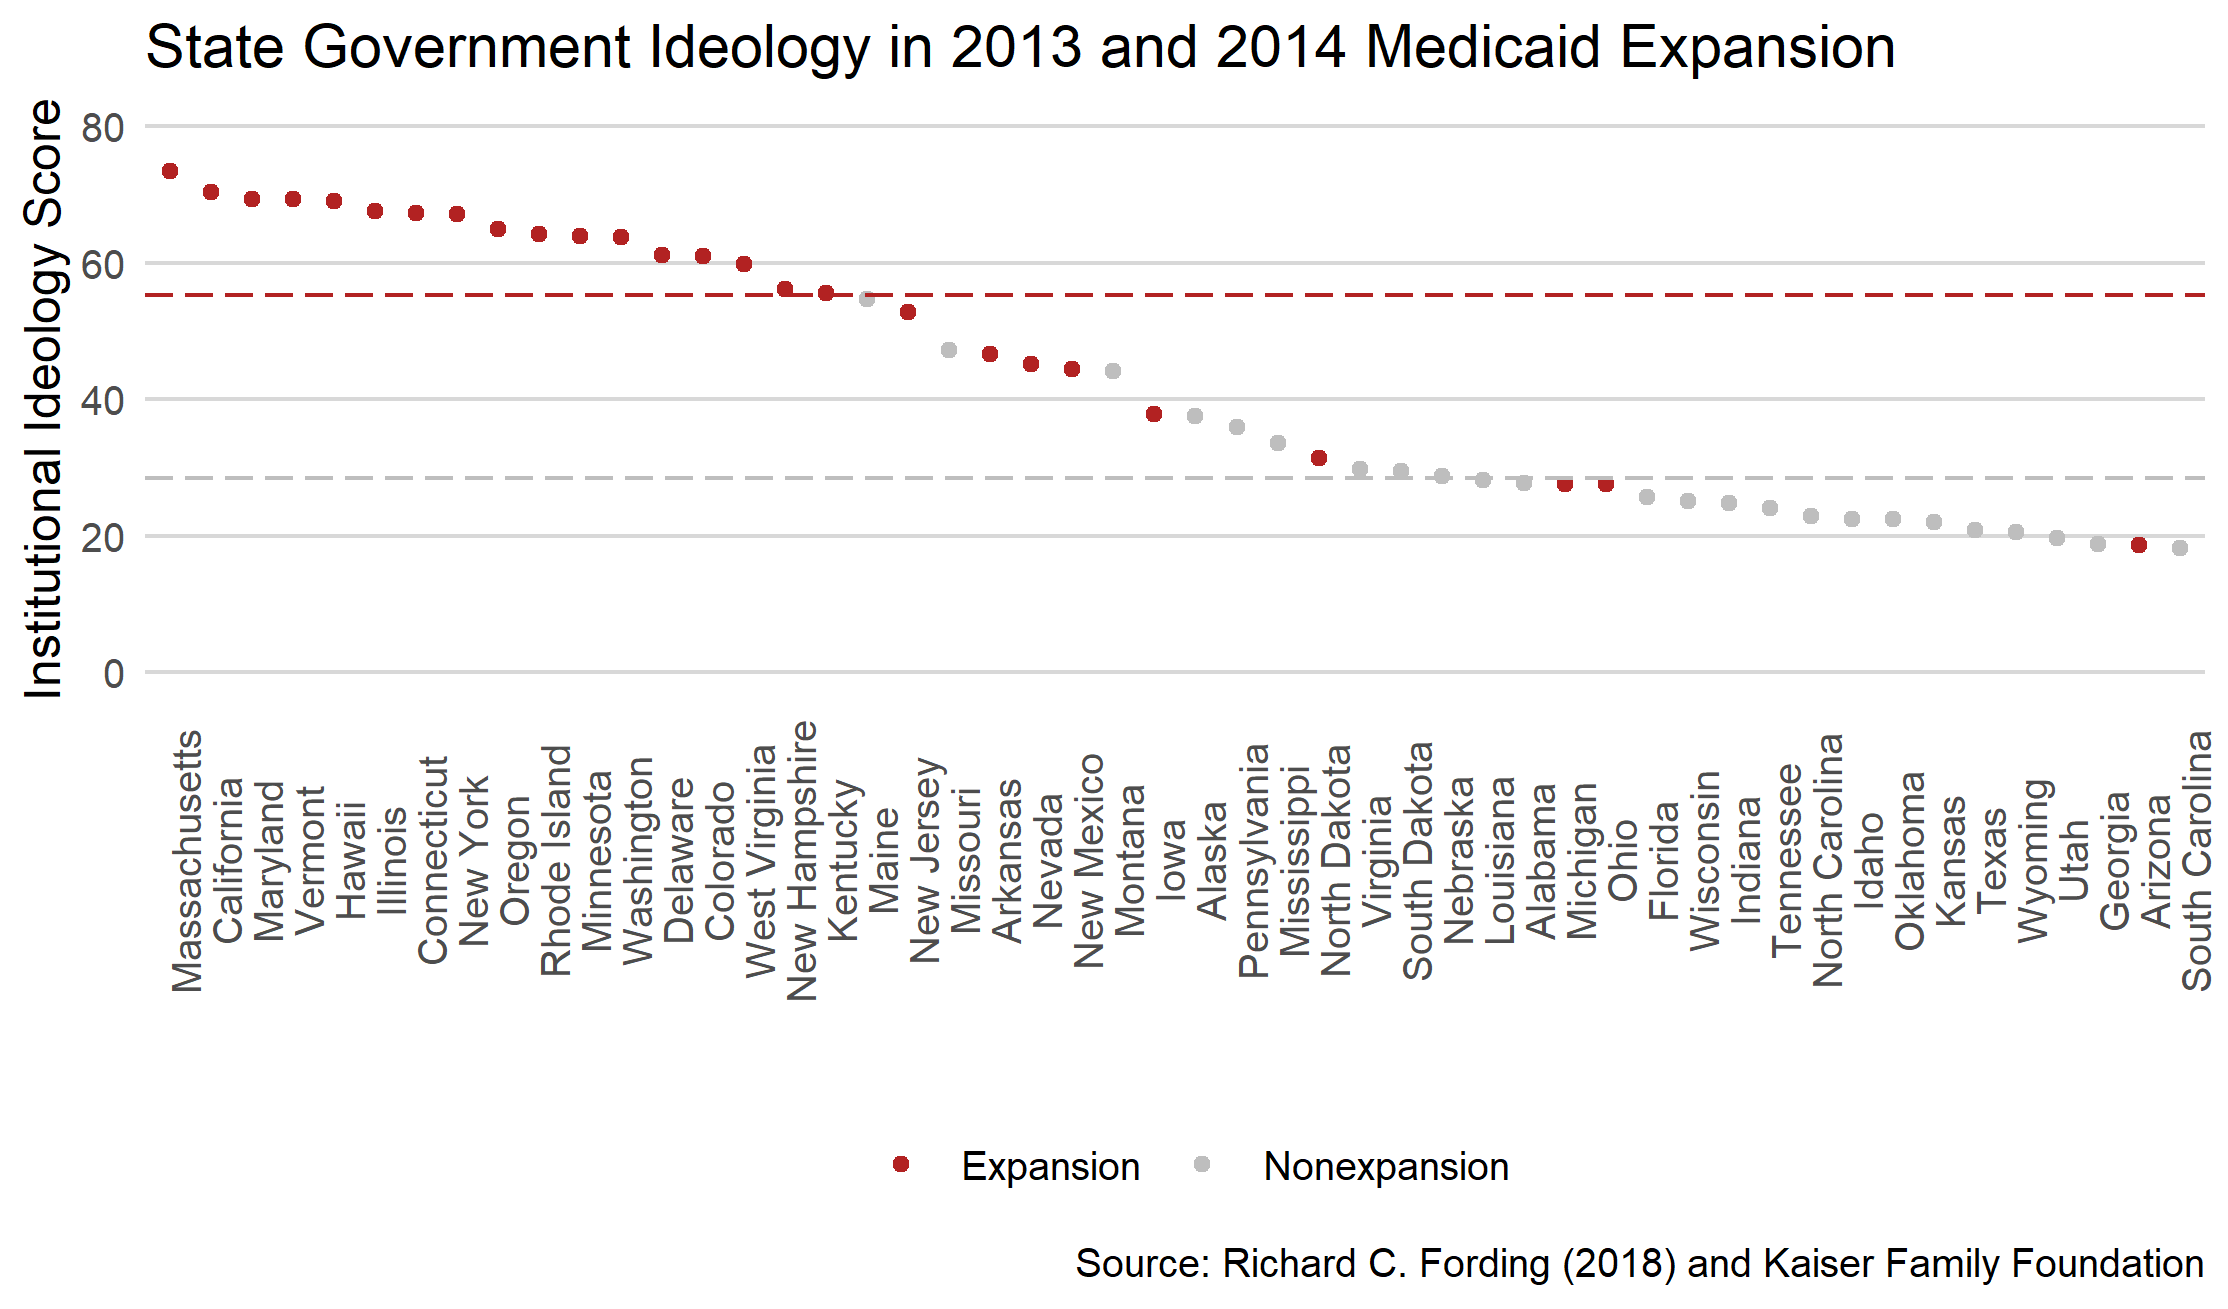
\includegraphics[scale=0.7]{images/political-expansion-plot.png}
    \caption{Government ideology and Medicaid expansion}
    \label{fig1}
    \end{center}
\end{figure}

This paper makes several methodological contributions. First, we extend the ``synthetic controls'' framework to estimate the ETU and to clarify the required assumptions. While balancing on pre-treatment outcomes alone arguably suffices for some synthetic control applications (see, eg, \cite{botosaru2017role}), here we want to estimate treatment response. We therefore assume no unmeasured confounding given a rich covariate set and a linear and additive outcome model that accounts for all interactions between treatment and the covariates. Secondly, we use an implementation of Stable Balancing Weights (\cite{zubizarreta2015stable}) to estimate a set of positive weights to weight the expansion regions to approximately match the covariate distribution of the non-expansion regions. To account for remaining imbalances in the covariates, we also augment these weights with a regression-model following \cite{ben2018augmented}.

Our second contribution is to modify Stable Balancing Weights for this setting. In particular, the SBW objective performs well assuming independent data with no measurement error. However, we use data from the American Communities Survey (ACS) aggregated to the consistent public use microdata area (CPUMA) level. These regions nest within states, and using these smaller regions allows us to get better balance on our covariates. However, our as a result our data both has a hierarchical structure (regions within states) and, because our region-level covariates are estimated from underlying survey data, we also have measurement error in the covariates which may bias our treatment effect estimates. We propose a modification of the SBW objective function to account for the hierarchical nature of the data. We use the replicate survey weights provided in the ACS data to estimate the covariance matrix associated with this variability and use this information to correct for this bias. This is first study we are aware of that attempts to correct for sampling variability in the covariates when using balancing weights. 

The remainder of this paper has the following structure. Section II provides an overview of the data and defines the study period, outcome, covariates, and treatment. Section III discusses our methods, beginning by defining our target estimand, and then outlining our identification, estimation, and inferential procedures. Section IV presents our primary results and sensitivity analyses. Section V provides a brief discussion of the policy relevance of our findings, and Section VI contains a brief concluding summary of the paper. Supplemental materials may be found in the Appendices.

\section{Data}

Our data source is the annual household and person public use microdata files from the American Community Survey (ACS) from 2011 through 2014. The ACS is an annual survey of approximately three million individuals across the United States; the public use files include information on individuals in geographic areas greater than 65,000 people. The smallest geographic unit contained in these data are public-use microdata areas (PUMAs), arbitrary boundaries that nest within state but not within counties or other more commonly used geographic units. One limitation of these data is a 2012 change in the definition of PUMA boundaries; moreover, these new boundaries overlapped with the previous boundaries. As a result, the smallest possible geographic areas that nest both PUMA coding systems are known as consistent PUMAs (CPUMAs). The United States contain 1,075 total CPUMAs, with states ranging from having one CPUMA (South Dakota, Montana, and Idaho) to 123 CPUMAs (New York). The total number of sampled individuals per CPUMA in any year in our study ranged from 531 (representing an area of approximately 96,000 individuals) to 49,046 (representing over 4.5 million individuals). The median sample size for a given CPUMA across the four years of our study is XXX.

\subsection{Study period}

We begin our analysis in 2011 following \cite{courtemanche2017early}, who note that several other aspects of the ACA were implemented in 2010 -- including the provision allowing for dependent coverage until age 26, and the elimination of co-payments for preventative care -- likely induced differential shocks across states. We also restrict our post-treatment period to 2014 only: several additional states expanded Medicaid in 2015, including Indiana, Michigan, and Pennsylvania. However, these states did not expand Medicaid contemporaneously with the 2014 ACA provisions. Without additional assumptions, this second-year expansion therefore represents a different causal estimand. 

\subsection{Covariates}

We use the underlying individual-level ACS survey data and accompanying survey weights to aggregate the data at the CPUMA level. We choose our covariates to approximately align with those considered in \cite{courtemanche2017early} and that we argue plausibly include all potential confounders in the outcome model. Because we are ultimately interested in calculating rates, these variables include both counts that we use for the numerators and denominators of the corresponding rates. 

The denominator counts include: total non-elderly adult population for each year 2011-2014; total labor force for each year 2011-2013; and the total number of households averaged from 2011-2013. We then calculate the total number of females; total number of whites; total number of people born outside of the United States; total number of citizens; total number with less than high school education, high school degrees, some college, or college graduates or higher; the total number living under 138 percent of the federal poverty line (FPL), between 139 and 299 percent, 300 and 499 percent, and more than 500 percent of the FPL; and the total number aged 19-29, 30-39, 40-49, 50-64. We then average these counts from 2011-2013. We also calculate the total number of households with one or more children among all households (averaged from 2011-2013). For each year from 2011-2013 we calculate the total number of unemployed individuals among the total number in the labor force and the total number of uninsured individuals among the non-elderly adult population. We then use Census data to calculate the approximate percentage of people living within an ``urban'' area for each CPUMA (\cite{census}). Finally, we include three state-level covariates reflecting the partisan composition of each state's government in 2013. Specifically, we include an indicator for having a Republican governor, an indicator for Republican control over the lower legislative chamber, and an indicator for Republican control over both chambers of the legislature and the governorship.\footnote{Nebraska is the only state with a unicameral legislature; moreover, the legislature is technically non-partisan. We nevertheless classified them as having a Republican control of the legislature.} 

\subsection{Outcome}

Our primary outcome of interest $Y$ is the non-elderly adult uninsurance rate in 2014. We might consider take-up rates among the Medicaid-eligible population to be a more natural outcome. However, we choose the non-elderly adult uninsurate rate for two reasons, one theoretic and one practical. First, Medicaid eligibility in the post-period is likely endogenous: Medicaid expansion may affect an individual's income and poverty levels, which define Medicaid eligibility. A second reason is to align our study to compare our results with the existing literature, and this is the outcome that \cite{courtemanche2017early} use. One drawback of using this outcome is that the simultaneous adoption of other ACA provisions in 2014 more clearly affects this rate in a way that a more targeted group might not.

\subsection{Treatment assignment}

While some states expanded Medicaid and other states did not, in reality assigning a binary treatment status simplifies a more complex reality. We note three reasons we should be cautious about this simplification. First, states differed substantially in pre-existing Medicaid coverage policies: with perfect data we might consider Medicaid expansion as a continuous treatment with values proportional to the number of newly eligible individuals. The challenge though is correctly identifying newly eligible individuals in the data (see \cite{frean2017premium}, who attempt to address this). Second, \cite{frean2017premium} note that six states adopted partial limited Medicaid expansions prior to 2014: specifically, California, Connecticut, DC, Minnesota, and New Jersey. \cite{kaestner2017effects} and \cite{courtemanche2017early} also consider Arizona, Colorado, Hawaii, Illinois, Iowa, Maryland, and Oregon to have had early expansions. Lastly, timing is an issue: among the states that expanded Medicaid in 2014, Michigan's expansion did not go into effect until April 2014, while New Hampshire's expansion did not occur until September 2014.

Our primary analysis excludes New York, Vermont, Massachusetts, Delaware, and the District of Columbia from our pool of expansion states, because these states had comparable Medicaid coverage policies prior to 2014 (\cite{kaestner2017effects}). We also exclude New Hampshire because it did not expand Medicaid until September 2014. While Michigan expanded Medicaid in April 2014, we leave this state in our treated pool. We consider the remaining expansion states as ``treated'' and the non-expansion states as ``control'' states. We later consider the sensitivity of our results to these classifications by removing the early expansion states noted by \cite{frean2017premium}. Our primary classification of expansion and non-expansion states is unique among similar studies: \cite{courtemanche2017early} classifies all expansion states as treated, and all non-expansion states as control. \cite{frean2017premium} exclude Massachusetts from expansion states. Lastly, \cite{kaestner2017effects} include Delaware, DC, Massachusetts, New York, and Vermont as control states. Our final dataset contains aggregated counts for all of the above variables for 925 CPUMAs in our non-expansion and our pool of expansion states. 414 CPUMAs were in non-expansion states and 511 CPUMAs were in expansion states.

\section{Methods}
\label{sec:methods}

In this section we formally present our causal estimand, our identification and estimation strategies, and our inferential procedure.

\subsection{Estimand}

We seek to estimate the average effect of 2014 Medicaid expansion would have had on the non-elderly adult uninsurance rate in states that did not expand Medicaid. Importantly, we condition on the observed treatment assignment and treat this variable as fixed in our analysis. The 2014 Medicaid expansion occurred simultaneously with the implementation of several other major ACA provisions, including (but not limited to) the creation of the ACA-marketplace exchanges, the individual mandate, health insurance subsidies, and community-rating and guaranteed issue of insurance plans (\cite{courtemanche2017early}). Almost all states broadly implemented these reforms beginning January 2014. Conceptually we think of the other ACA components as a treatment ($V$) separate from Medicaid expansion ($A$).

Let $i$ index a CPUMA, $j$ index the state, $t$ index the time period, and let $Y_{ijT}^{A_{ijT} = a, V_{ijT} = v}$ be the potential number of uninsured given Medicaid expansion and other ACA-reforms at time $T = 2014$. We consider the case where these potential outcomes are deterministic: that is, given any state of the world $A = a, V = v$, a CPUMA has some fixed potential uninsurance rate. We then wish to estimate the following contrast:

$$
\psi = \sum_{i: A_{ijT} = 0, V_{ijT} = 1} Y_{ijT}^{A_{ijT} = 1, V_{ijT} = 1} - Y_{ijT}^{A_{ijT} = 0, V_{ijT} = 1} 
$$

In other words, we want to estimate the difference in the total number of uninsured non-elderly adults among states that did not expand Medicaid, but did implement other aspects of the ACA. Because all states implemented the ACA marketplace expansion in 2014, contrasts with the corresponding potential outcome absent this expansion are not identified. Moreover, since we are only interested in the counterfactual at time $T$, we simplify notation by removing this variable and the subscript in the estimand:

$$
\psi = \sum_{ij: A_j = 0} Y_{ij}^{A_{ij} = 1} - Y_{ij}^{A_{ij} = 0}
$$

We therefore seek to identify the effect of Medicaid expansion in the context of the simultaneous implementation of the ACA, but do not attempt to separately identify the effects of these separate treatments. Notice that because non-expansion states were subject to an intervention the post-treatment period, in contrast to other panel data settings, we never observe $Y_{ijT}^{A_{ij} = 0, V_{ij} = 0}$. Because we assume that interactions between the ACA implementation and Medicaid expansion may vary over time, we do not seek to generalize these results outside of 2014. 

\subsection{Identification}

We make the following causal assumptions: consistency, no unmeasured confounding, no anticipatory treatment effects, and positivity of treatment assignment. Consistency states that the observed factual outcome under a given treatment assignment is equal to the potential outcome under that same treatment assignment ($Y_{ij}^{A_{ij} = a} = Y_{ij} \mid A_{ij} = a$). In other words, we assume that one regions' treatment assignment didn't affect another regions' observed outcome. This assumption is standard throughout the literature, but is often not realistic. Violations of this assumption are likely in our study: for example, \cite{frean2017premium} find evidence that Medicaid expansion drove previously eligible but uninsured individuals to enroll in Medicaid in both expansion and non-expansion states. Signing the potential bias from these spillovers requires redefining the causal estimand: for example, we might consider the treatment effect on the untreated given that all states have expanded Medicaid, where the contrast is against where only the observed expansion states expanded Medicaid (ie $N_c^{-1}\sum_{ij: A_j = 0}(Y_{ij}^{A_1 = ... = A_{N_t} = 1, A_{N_t + 1} = ... = A_{N_t + N_c} = 0} - Y_{ij}^{A_1 = ... = A_N = 1}$). If spillovers occurred in equal proportions in each region, and the magnitude of the spillovers increase with the number of treated regions, then the true effect would be larger in absolute magnitude than the effect estimated using the observed data. We could consider other estimands or assumptions to get different predictions about the sign of the bias, but we leave this as an area for future work.

We next assume that there were no anticipatory treatment effects. Letting treatment occur at time $T_0 + 1$, we have that for $t \le T_0$

$$
Y_{ijt} = Y_{ijt}^0
$$

This assumption is necessary because we are conditioning on pre-treatment outcomes. If these outcomes were affected by the treatment before it were implemented, these covariates would not be exogenous. Anticipatory treatment effects may occur if plans to expand Medicaid induce uninsured but Medicaid-eligible individuals to enroll in Medicaid prior to expansion. We do not think these violations occurred in large enough numbers to substantially affect our results. Instead, we address a more concerning version of this violation: as noted above, several states allowed certain counties to expand Medicaid prior to 2014. We therefore test the sensitivity of our results to the inclusion of these states.

Third, we assume no unmeasured confounding; that is, that at time $T$ the potential outcomes for each CPUMA are independent of the state-level treatment assignment conditional on the true CPUMA and state-level covariates $X_{ij}$ (which includes pre-treatment outcomes):

$$
Y_{ij}^a \perp A_{ij} \mid X_{ij}
$$

While unverifiable, we believe it is reasonable here given our rich covariate set. To be explicit, we believe that the uninsurance rate for each region given treatment is independent of the region's treatment assignment conditional on the percentage of uninsured individuals in the pre-treatment period, the percentage of unemployed individuals in the pre-treatment period, the population growth in 2012 and 2013, the average ratio of households to total population, the state's political composition, the average proportion of households with one or more children during the pre-treatment period, and the average proportion of individuals during the pre-treatment period with given demographics noted above (age, sex, white, hispanic, US citizenship, foreign born, income-to-poverty group, disability status, urban residence, and educational attainment group). If this assumption were violated -- that is, other covariates exist that determine this potential outcome and treatment assignment -- we hope that conditioning on pre-treatment outcomes might help proxy for these covariates, thereby minimizing the potential for bias. 

Having said that, we do not actually observe the true values of $X_{ij}$ but rather an estimate $W_{ij}$. Importantly, $Y_{ij}^a \perp A_{ij} \mid X_{ij} \not\implies Y_{ij}^a \perp A_{ij} \mid W_{ij}$. Therefore, the use of these proxies may also bias our estimates. We rely on several modeling assumptions outlined below in our estimation procedure to correct for this bias.

Finally, we assume positivity of treatment assignment; that is, that all states had some probability of being treated $\pi(X_{1j}, ..., X_{n_jj}) > 0$. Positivity violations can cause a lack covariate overlap in the observed data. As we have noted before, overlap is an issue in this study, which we address in our estimation strategy, outlined below.

The above assumptions give us non-parametric identification of our causal estimand. We make the further parametric assumptions that the outcome under treatment is linear and additive in the covariates $X_{ij}$ (notice that because we observe $Y_{ij}^0$ for the control units, we do not need to specify a model of $\mu_0$; instead, we simply take the mean of the observed values to estimate $\sum_{i: A_{ij} = 0} Y_{ij}^{A_{ij} = 0}$). Specifically, we believe that the following model generates the potential non-elderly adult uninsurance rate under treatment:

$$
\mu_1(X_{ij}) = \mathbb{E}\{Y_{ij} \mid X_{ij}, A_{ij} = 1\} = X_{ij}^T\beta
$$

This contrasts with the synthetic controls literature, where a commonly invoked motivation is that the outcome model absent treatment ($\mu_0(X_{ij})$) follows an interactive fixed effects model (see, eg, \cite{abadie2010synthetic}, \cite{ben2018augmented}). That model instead posits that pre-treatment outcomes can act as proxies for a form of time-varying unobserved confounding. Nevertheless, these causal and parametric assumptions are sufficient to allow us to estimate the treatment effect. 

\subsection{Estimation}

We outline our estimation strategy emphasizing first how our method differs from the synthetic controls approach. In particular, we explain why our approach must rely on stronger modeling assumptions than synthetic controls applications and why we therefore choose to use an implementation of Stable Balancing Weights (SBW) for our modeling. Second, we explain the modifications we make to the SBW objective (which we call H-SBW), how they reduce the variance of our estimator given our hierarchical data structure, and how they result in a consistent estimate under measurement error in the covariates. Finally, we explain how due to remaining imbalances in our covariates, we debias our estimator using ridge-augmented weights, following the suggestion of \cite{ben2018augmented}.

Similar to synthetic controls applications, we seek to generate a set of positive weights that balance the means of the treated units to the mean of the control units. Assume that we observe the true covariates $X_1$ and $X_0$, and let $\bar{X}_0^p_x$ be the (population-weighted) average of the covariate values in the non-expansion region. Ideally, we could then find some $\gamma^\star$ such that: 

$$
(N_t^{-1})X_1^T\gamma^\star = \bar{X}_0^p, \gamma_i^\star > 0, \sum_{ij} \gamma_{ij}^\star = N_t
$$

Let $p$ be a vector of (normalized) population weights for each CPUMA in the non-expansion region in year $T = 2014$. We could then estimate $\psi$ as

$$
\hat{\psi}^{\gamma} = (N_t^{-1}\sum_{j: A_j = 1}^{M_t}\sum_{i = 1}^{n_j}\gamma_{ij}^\star Y_{ij} - \sum_{j: A_j = 0}\sum_{i = 1}^{n_j}Y_{ij}p_{ij})
$$

Using our assumption that $\mu_1(X_{ij}) = X_{ij}^T\beta$, the bias of our estimator $\mathbb{E}\{\hat{\psi}^w - \psi^w\}$ is less than or equal to $\beta^T \delta = \beta^T(X_1^T\gamma - \bar{X}_0^p) = 0$ (see, eg, \cite{zubizarreta2015stable}). The challenge, however, is that for any given dataset we have no guarantee that any such $\gamma$ exists that exactly balances the covariates; we therefore need some method of determining how to prioritize which parts of the covariate distribution we wish to balance.

This is where our method to estimate the ETU contrasts with the commonly used synthetic control approach used to estimate the ETT: \cite{abadie2010synthetic} determine how to prioritize covariate balance by training their model on pre-treatment outcomes (\cite{kaul2015synthetic} shows that often the most relevant covariates simply become the pre-treatment outcomes). Because in that setting $Y^0_{ijt}$ is actually observed for $t \le T_0$, \cite{abadie2010synthetic} leverage this data to select the covariates that best predict these values. By contrast we never observe $Y^1_{ijt}$ prior to treatment. Without additional assumptions, we cannot use the pre-treatment data to learn which covariates matter most for determining this potential outcome.

Moreover, the problem of predicting treatment response also makes estimating the ETU more challenging than the ETT. As a result, we may care far more about balancing ``auxillary covariates'' (ie covariates that are not pre-treatment outcomes) in our setting than the traditional synthetic controls setting.\footnote{Recent discussions in the synthetic controls literature often prioritize discussing balancing pre-treatment outcomes alone (see, eg, \cite{doudchenko2016balancing}). This has some theoretic justification: \cite{botosaru2019role} find that when a sufficiently large amount of pre-treatment outcomes, assuming $\mu_0$ follows a linear factor model, the bias of the estimator is still bounded even if imbalances in auxillary covariates remain.} Consider the following example: say for some application there exist two sets of weights, $\gamma_1$ and $\gamma_2$, that exactly balances $k$ pre-treatment means of the controls units to the treated unit(s). $\gamma_1$ additionally exactly balances $p$ auxillary covariates, while $\gamma_2$ does not. Heuristically, estimates using either set of weights may provide reasonable counterfactuals for the treated unit(s) absent treatment. However, once we invert the treatment assignment -- ie the control units are treated and the treated units control -- and consider predicting the outcome under treatment: intuitively, we should choose $\gamma_2$. Why? Because we might worry that these observable characteristics predict treatment response, and the treatment response of these two units might differ substantially. 

More formally, assume that $\mu_0(X_{ij})$ follows a linear outcome model. We might reasonably believe the coefficients on auxillary covariates are close to zero once we condition on pre-treatment outcomes. As a result, the bias induced by imbalances on these covariates would be small. On the other hand, the coefficients on the same covariates for the model $\mu_1(X_{ij})$ could be much larger, even after conditioning on pre-treatment outcomes. If our synthetic control weights fail to balance these covariates, we should expect that our estimates of $\mu_0$ will in general have less bias than our estimates of $\mu_1$. In summary, estimating the ETU requires a greater understanding of how the covariates are related to treatment response than the ETU; moreover, and we cannot learn this information by using pre-treatment outcomes.

We therefore estimate the ETU by using a variation of SBW proposed by \cite{zubizarreta2015stable}.\footnote{Specifically, we use a modified implementation of Noah Griefer's ``optweight'' package in R, available on github.com/mrubinst757}. This procedure allows us to estimate the minimum variance weights that satisfy certain balance constraints. Letting $X_1$ and $X_0$ be the matrices of the observed treatment and control group covariates (and dropping the subscript $t$ for notational convenience), we generate weights that solve the following objective:

$$
\min_{\gamma \in \Gamma} \sum_{ij: A_j = 1} \gamma_{ij}^2 + \sum_{kj \ne ij}\rho \gamma_{ij}\gamma_{kj}
$$

$$
\Gamma := \{\gamma: \mid N_t^{-1}\hat{\mathbb{E}}\{X_1 \mid W_1\}^T\gamma - \bar{X}_0^p \mid \le \delta, \gamma_{ij} > 0, \sum_{ij}\gamma_{ij} = N_t\}
$$

Unlike the synthetic controls objective, the SBW objective allows the user to specify covariate-level balance constraints as a tuning parameter $\delta_d$. When estimating the ETU, we lean heavily on assumptions to justify our choice of $\delta$; in particular, we use a priori knowledge about which covariates are most likely to be important predictors of treatment effect heterogeneity when setting $\delta$. 

We now discuss our modifications to the SBW objective function. Recall that the SBW criterion is equivalent to ours when setting $\rho = 0$; in other words, SBW attempts to calculate the minimum variance weights for a fixed $\delta$. This is desirable if, for example, the errors in our outcome model are all independent and identically distributed. In our case, we account for possible state-level dependencies in the outcome model (or, alternatively, depending on one's viewpoint, state-level sampling or state-level treatment assignment). Intuitively, by adding the tuning parameter $\rho$, this objective attempts to ensure that the within state sum of weights is roughly uniform across states as well as across CPUMAs. This is especially desirable if many weights would in some cases be concentrated in only one state. We discuss this objective in more detail and provide simulation results in Rubinstein (2020) (not yet publicly available).

Secondly, we do not balance on the observed covariate values $W_{ij}$, but rather on our estimate of $\mathbb{E}\{X_{ij} \mid W_{ij}, A_j = 1\}$. This is because the estimation error in these region-level estimates will bias our estimator. In the Appendix, we prove that this bias is equivalent to the bias induced in the classical measurement error problem using OLS. We therefore use regression-calibration techniques (see CITE). Specifically, we are able to use the person-level replicate survey weights provided in the ACS microdata to generate 80 additional CPUMA-level datasets. We then use these datasets to estimate the variability in each CPUMA's observed covariate values. Using these estimates of the errors, we are able to construct a linear approximation to the true covariate values. CITATION. We gives further details about our calibration procedure in the Appendix. The consistency of this estimator follows from existing results on linear models. 

This is the first application we know of to use these measurement error corrections in the context of balancing weights. We emphasize the key assumptions for the theoretical groundings for this procedure: (1) the outcome model is linear in the covariates; (2) the measurement error in the outcome is unrelated to the measurement error in the covariates; (3) the covariates as randomly sampled from some larger super-population. Taking the fixed-design approach seems more natural here, as we might consider the states we observe to be our population. This assumption is not strictly necessary; regression-calibration techniques have shown to perform well under fixed-design settings as well. SEE EG CITE. We believe the second assumption is reasonable here because the outcome is estimated from a different cross-section of the ACS than the covariates. Finally, the linearity and additivity assumptions are quite strong, though standard in many applications.

Lastly, we are unable to achieve exact balance on our covariates. This could potentially bias our estimator. Following the recent literature on synthetic controls, we reduce this bias by using ridge-regression augmented weights \cite{ben2018augmented}. Letting $Z_{ij} = \hat{\mathbb{E}}\{X_{ij} \mid W_{ij}\}$, we use regression-augmented weights:

$$
\gamma^{aug} = \gamma^{sbw} + (Z_1^T\gamma - \bar{W}_0^p)^T(Z_1^T\Omega^{-1}Z_1 + \lambda I_d)^{-1}Z_1^T\Omega^{-1}
$$

where $\Omega$ is a block diagonal matrix with diagonal entries equal to one and the within-group off diagonals equal to $\rho$. We choose $\lambda$ so that the remaining imbalances all fall within 0.1 percentage points (see \cite{ben2018augmented} for more details on the connection between these weights and ridge-regression). The cost of this procedure is that we must extrapolate from the support of the data, and therefore rely more heavily on our modeling assumptions. Finally, notice that we can also generate Oaxaca-Blinder weights ($\gamma^{ob}$) by setting $\gamma^{sbw} = 1/N_t$ and $\lambda = 0$. These are equivalent to running OLS (or GLS) on the observed outcomes among the treated units and imputing the missing counterfactual using these coefficient estimates. In our results we consider estimators using Stable Balancing Weights ($\rho \in \{0, 1\}$), and ridge-augmented versions of SBW and H-SBW. We also generate Oaxaca-Blinder weights setting $\rho \{0, 0.2\}$ and provide these results in the Appendix. We focus our discussion on our preferred estimators, H-SBW wand the ridge augmented version (BC-HSBW).

\subsection{Inference}

Inference with region-level panel data is a much studied topic, with many interesting ideas on how best way to think about and estimate randomness in this setting (see, eg, \cite{chernozhukov2017exact}). However, measurement error in the covariates is generally not assumed. We have the following sources of error in our estimator: (1) estimator error of the conditional expectation function $\mathbb{E}\{X_{ij} \mid W_{ij}\}$; (2) the difference in the true covariates from their expectation; (3) measurement error in the outcome; (4) model-based error in the outcome model; (5) our estimate of $Y_{ij}^1$. While regression calibration is motivated by the idea that $X_{ij}$ are random, we take the position that there are some true underlying covariate values. Regression calibration is shown in this setting to be an empirical Bayes approach to imputing the true covariates and is shown to have good performance. Therefore, the only source of variability in our estimates comes from the model-based error. Because we have counties within states, we have errors that in general decay at $1/sqrt{M_c}$ rates. (1) and (2) will bias our estimates, but we show in the Appendix that this bias is bounded in probability at smaller rates. We therefore expect that cluster-robust standard errors should have sufficient coverage of the true underlying parameter. 

\section{Results}

We present the analyses using our transformed covariates $Z_{ij} = \hat{\mathbb{E}}\{X_{ij} \mid W_{ij}, A_j = 1\}$. Figure \ref{loveplot} shows how our balancing weights reduce the imbalances in the covariates with the ten largest unweighted L1 differences. We see that our weights drastically reduce these differences; however, some imbalances remain. In particular, the Republican governance indicators are substantially imbalanced. A full balance table is available in the Appendix. 

We see...

\begin{figure}[B]
\begin{center}
    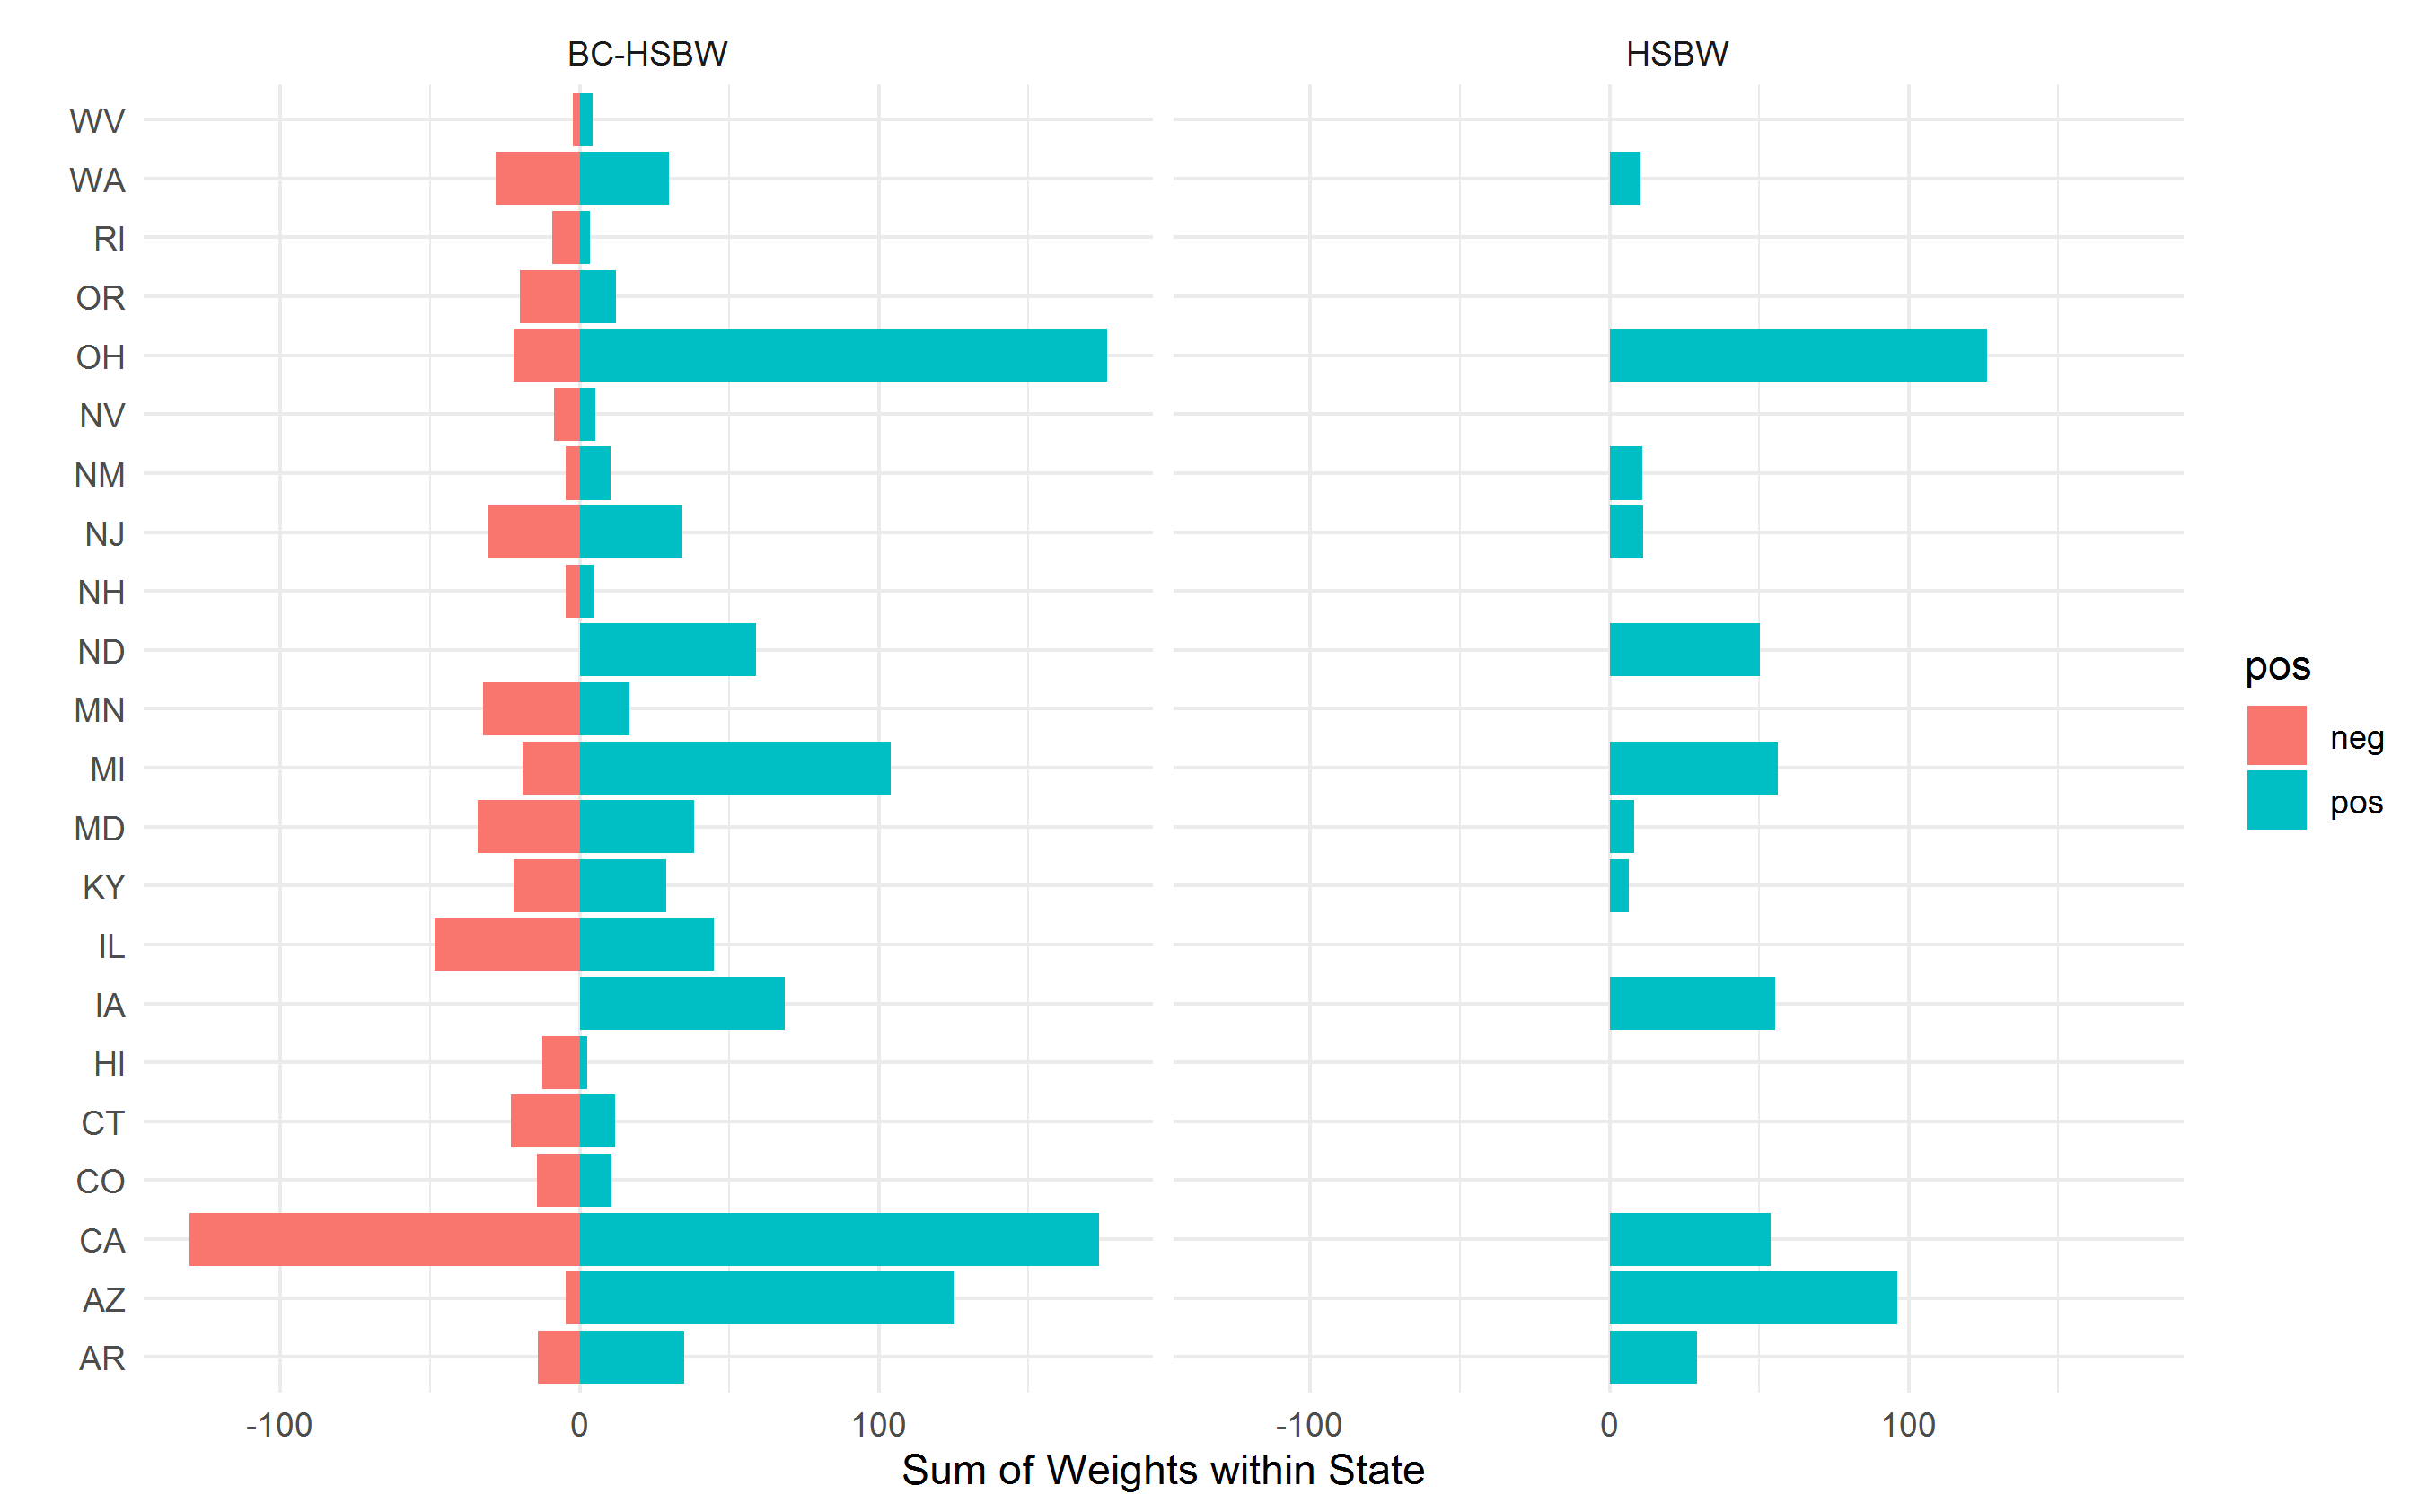
\includegraphics[scale=0.6]{01_Plots/weights-by-state-main.png}
    \caption{Total weights by State}
    \label{statewghts}
\end{center}
\end{figure}

We therefore use a ridge-augmentation to extrapolate from the data to reduce all imbalances within 0.1 percentage points. Figure \ref{statewghts} shows the total weights summed across states for each estimator: HSBW and BC-HSBW. This figure separately sums the negative weights from the positive weights to make clear the extent of the extrapolation. We see that BC-HSBW does extrapolate somewhat heavily in order to generate counterfactuals, particularly from California. 

Our H-SBW estimator yields an estimated effect of -1.89 (-0.86, -2.90).\footnote{This estimator ran the objective function above using $\rho = 0.2$ and imputing the covariates in the second procedure outlined in the Appendix.} In other words, had states that did not expand Medicaid done so, we would have seen a 1.89 percentage point reduction in their uninsurance rates in 2014. Encouragingly, the bias-correction makes almost no difference to the point estimate, although the confidence interval increases to (-0.79, -2.99). These estimates differ somewhat from the estimates we find running the procedure on the observed values $W_i$: here we calculate our preferred weighting estimator as -2.26 (-1.64, -2.87), and the bias corrected estimator yields -2.50 (-1.82, -3.17). Using the corrected dataset appears to both move our estimate closer in absolute magnitude towards zero and increase the estimated confidence intervals. This is expected because the imputation essentially shrinks outlying values of $W_i$ closer to $\bar{W}$; as a result, our weights must become more extreme in order to achieve the same level of covariate balance. Oaxaca-Blinder weights give an estimate of -1.58 (-0.83, -2.32); however, these weights extrapolate most heavily from the data of these three weight sets. Figure \ref{estimators} displays the point estimates from each of our weighting estimators. 

\begin{figure}[B]
\begin{center}
    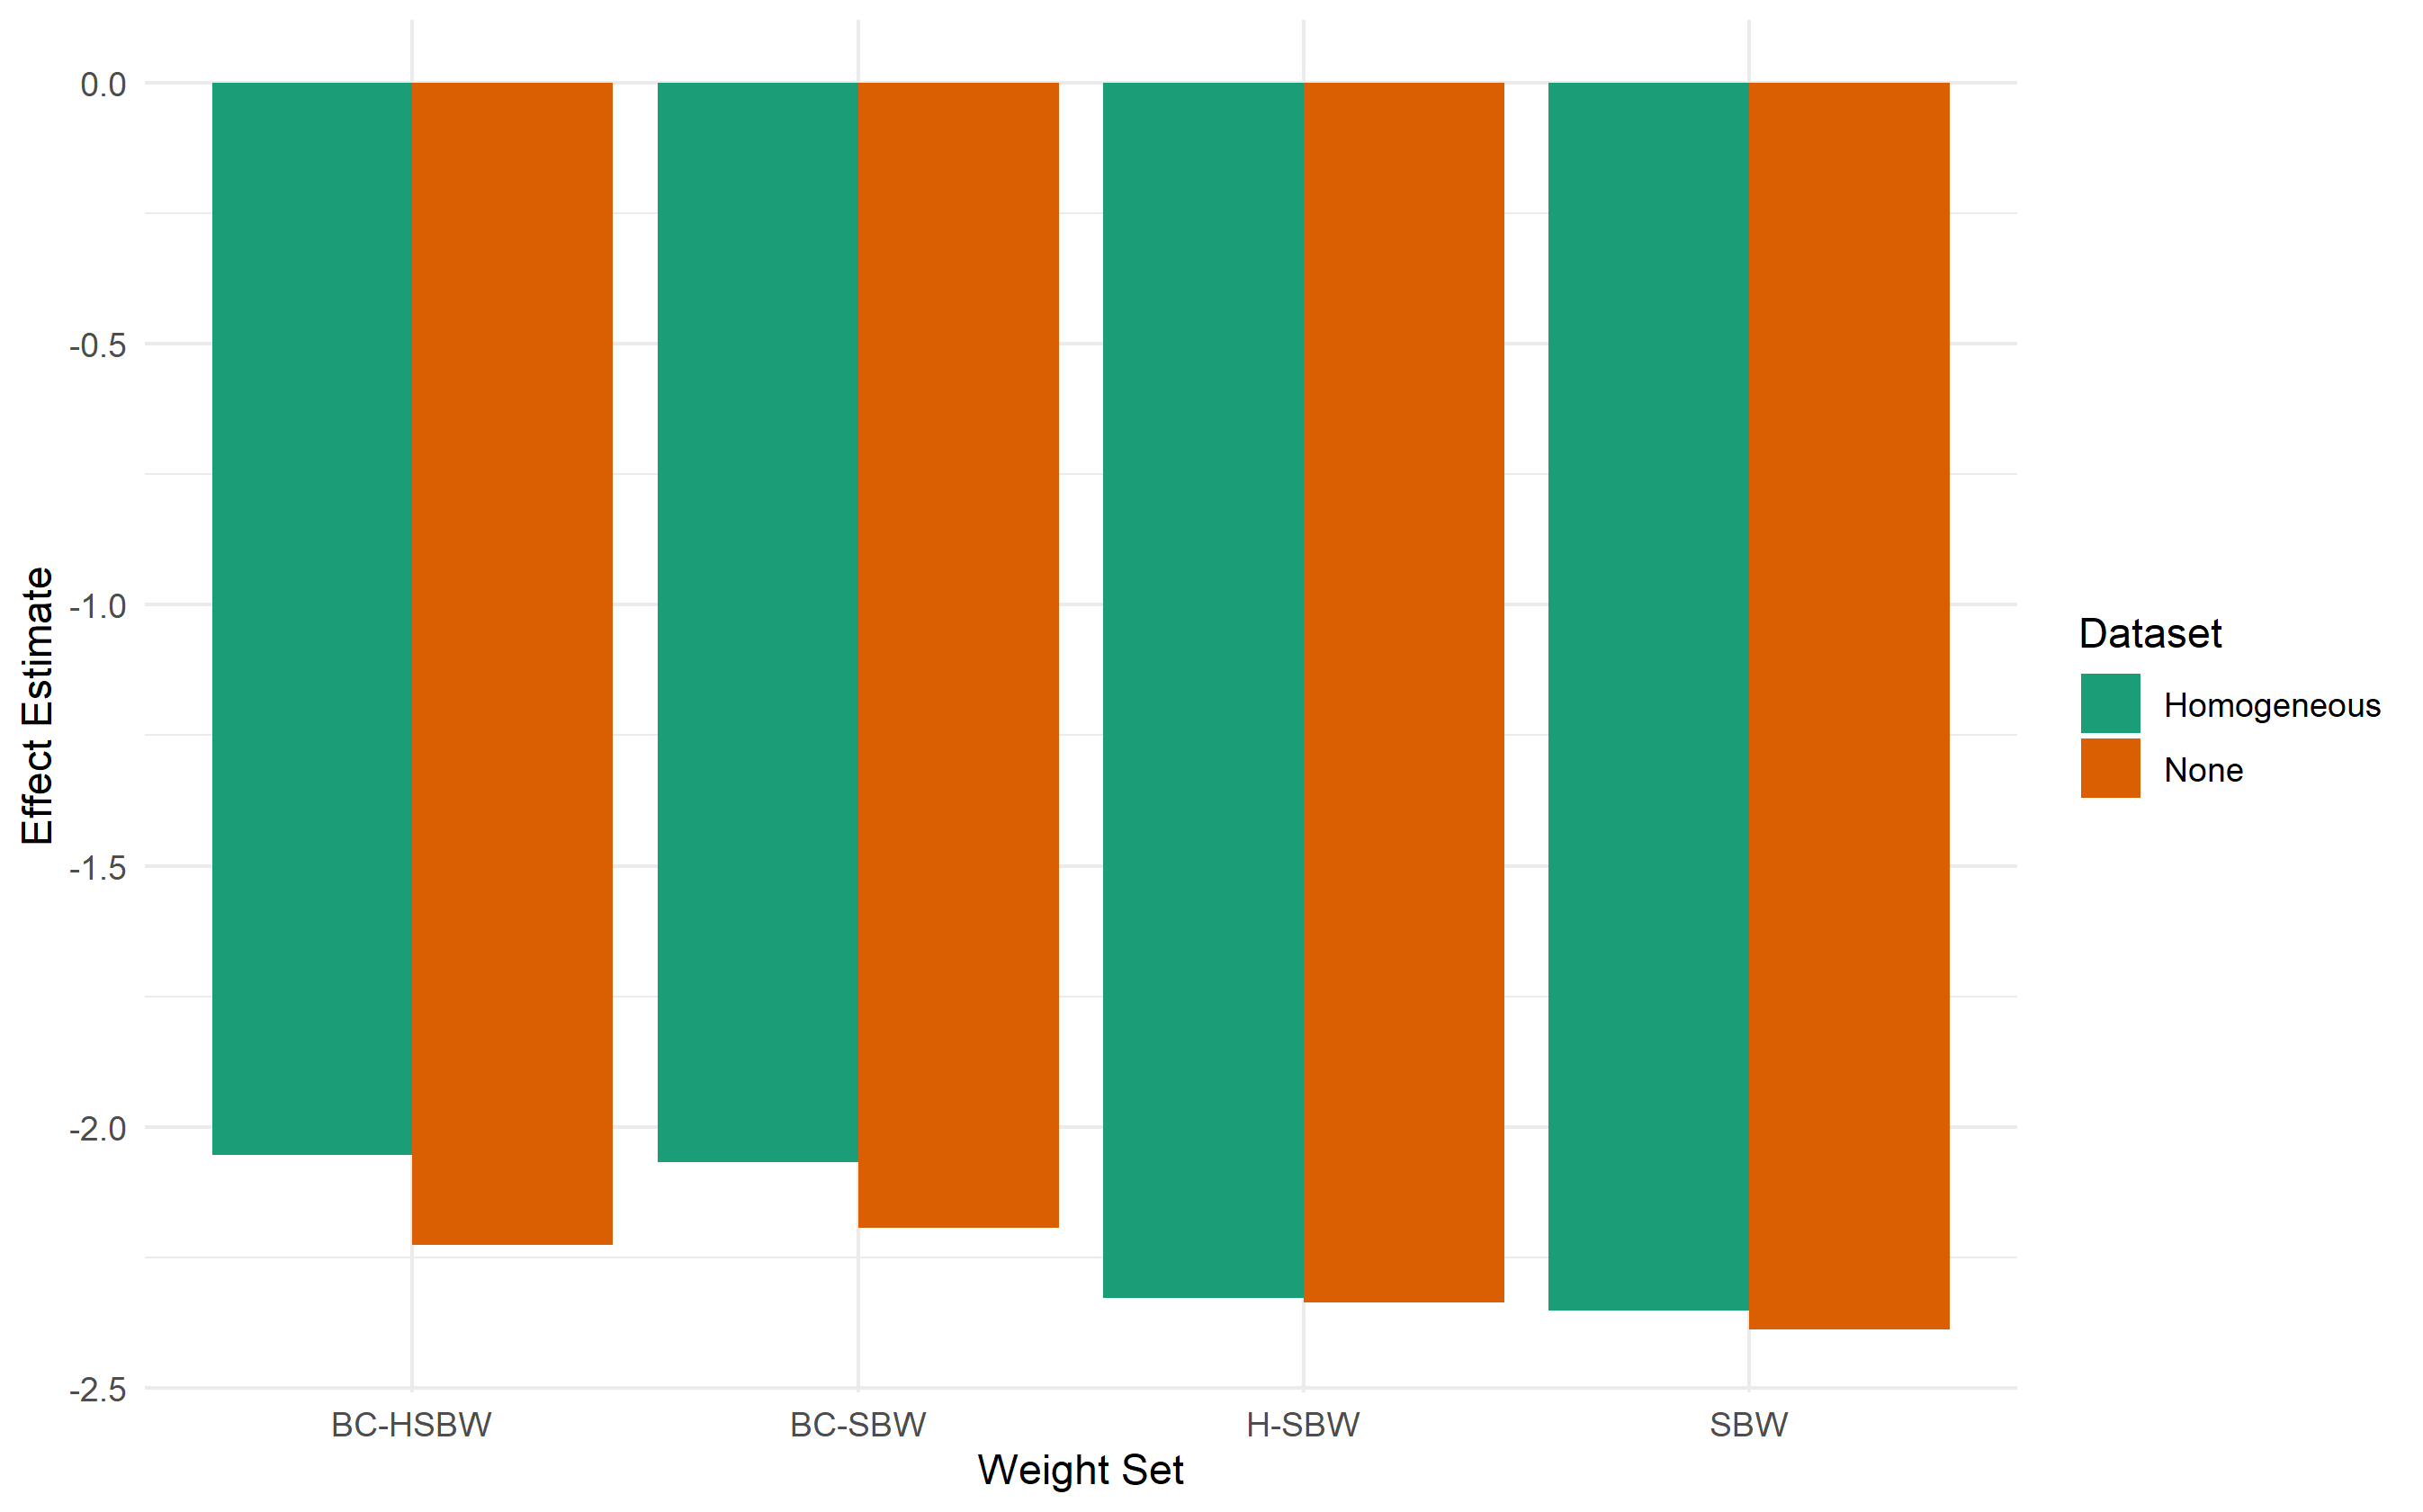
\includegraphics[scale=0.6]{01_Plots/point-estimates-c1.png}
    \caption{Point estimates by estimator}
    \label{estimators}
\end{center}
\end{figure}

We next examine how removing specific covariate groups in the weighting procedure changes the estimated contrast between the weighted treatment and control regions (ie the estimated treatment effect when all groups are included). We are especially interested how this contrast changes when we remove the Republican governance indicators: because we hypothesize that regions under Republican governed administrations should have lower Medicaid take-up rates, we expect that removing these covariates should move this estimate farther away from zero. We divide our covariates into six separate groups: pre-treatment uninsurance rates and pre-treatment unemployment rates, Republican governance indicators, and three sets of different demographic indicators.\footnote{Specifically, the first includes: urban residence, age group, education, citizenship, student, disability, female; the second, white race, hispanic, foreign-born, and income-to-poverty ratio bucks; the third, number of children, household to population ratio, and population growth.} We then rerun the analyses excluding each group. 

\begin{figure}[]
\begin{center}
    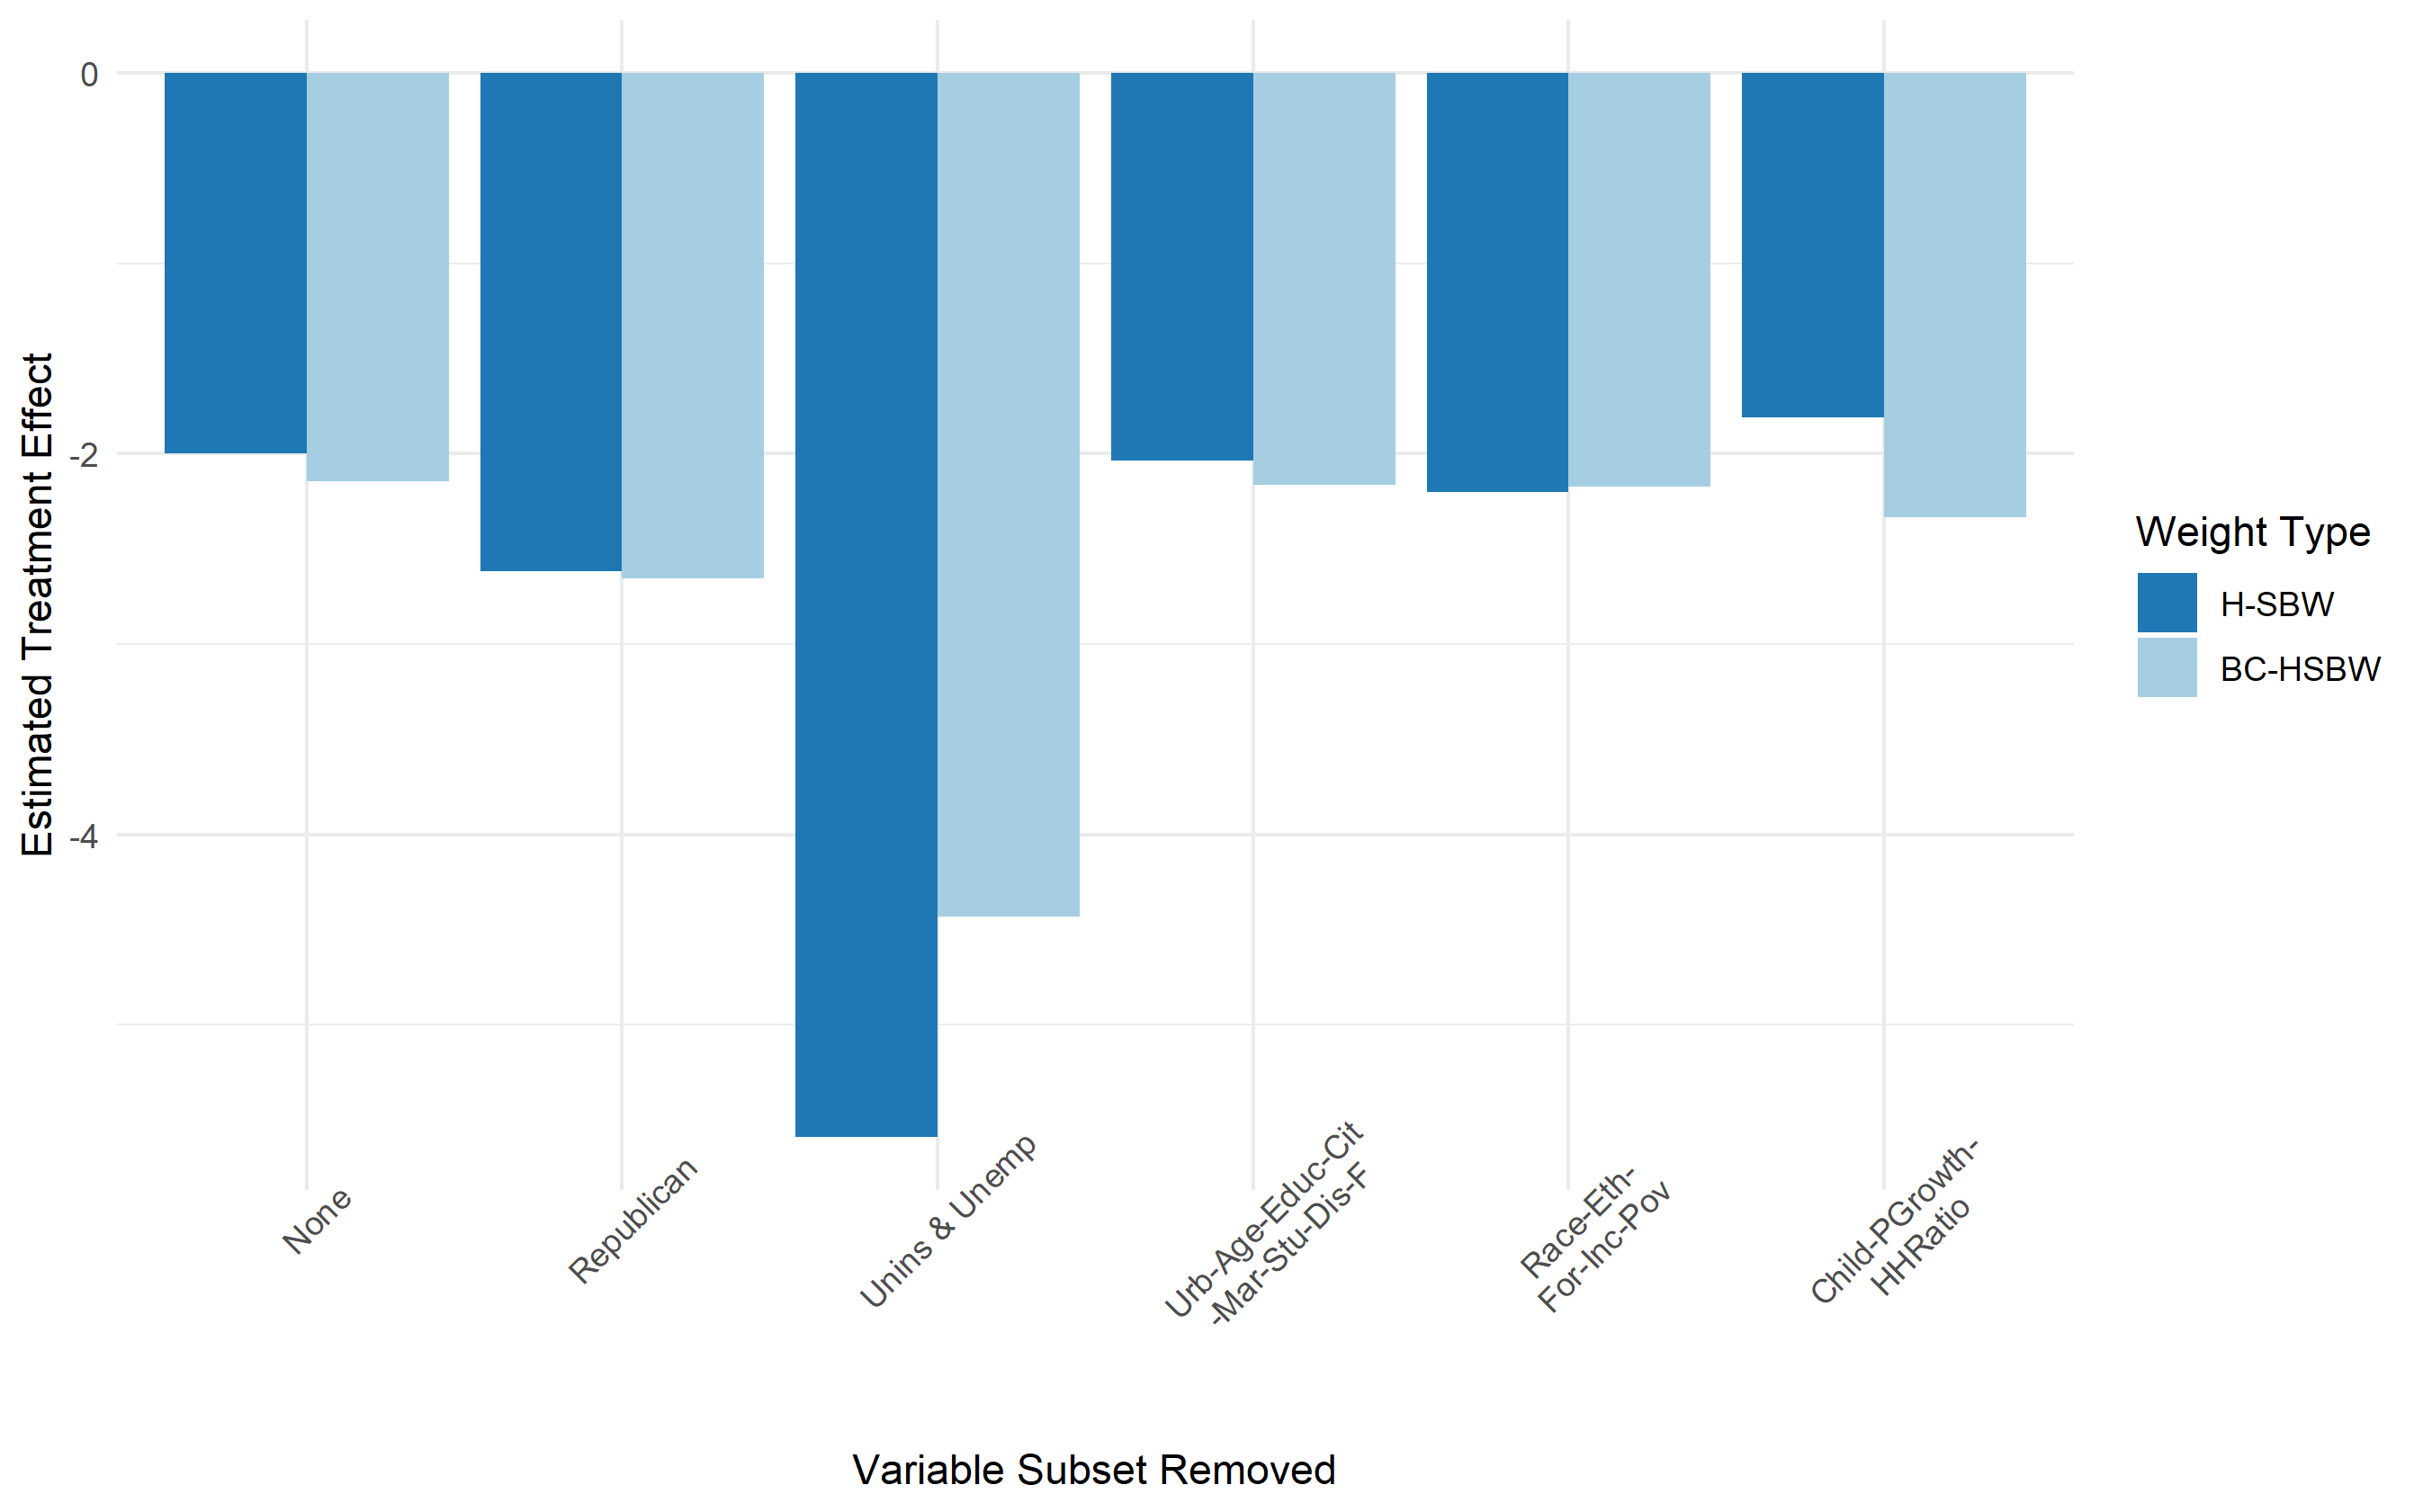
\includegraphics[scale=0.6]{01_Plots/loo-covariates-main-c1.png}
    \caption{Estimates}
    \label{loocovariates}
\end{center}
\end{figure}

Figure \ref{loocovariates} displays the estimated treatment effects when removing each covariate group for our preferred set of weights and the bias corrected version of these same weights. Unsurprisingly, we find that all our estimators are very sensitive to the removal of the vector of pre-treatment uninsurance and pre-treatment unemployment rates. When we fail to control for these covariates, our estimated contrast increases substantially in absolute magnitude. We also find that our preferred bias-corrected estimator is somewhat sensitive to the removal of children/population-growth/household ratio group. We do see that the OB weighting estimator is also sensitive to the removal of these covariates, though this does not occur with the SBW estimator (results available in the Appendix). 

Most importantly, we see a substantial increase in absolute magnitude of our estimated contrast when removing the Republican governance indicators. Specifically, we find that our estimated contrast increases in absolute magnitude by 0.65 for our preferred estimator and by 0.72 for our bias-corrected estimator. A similar differential also occurs on our unadjusted dataset. These results confirm our hypothesis that Republican governance drives heterogeneity in the treatment effects.

\begin{figure}[]
\begin{center}
    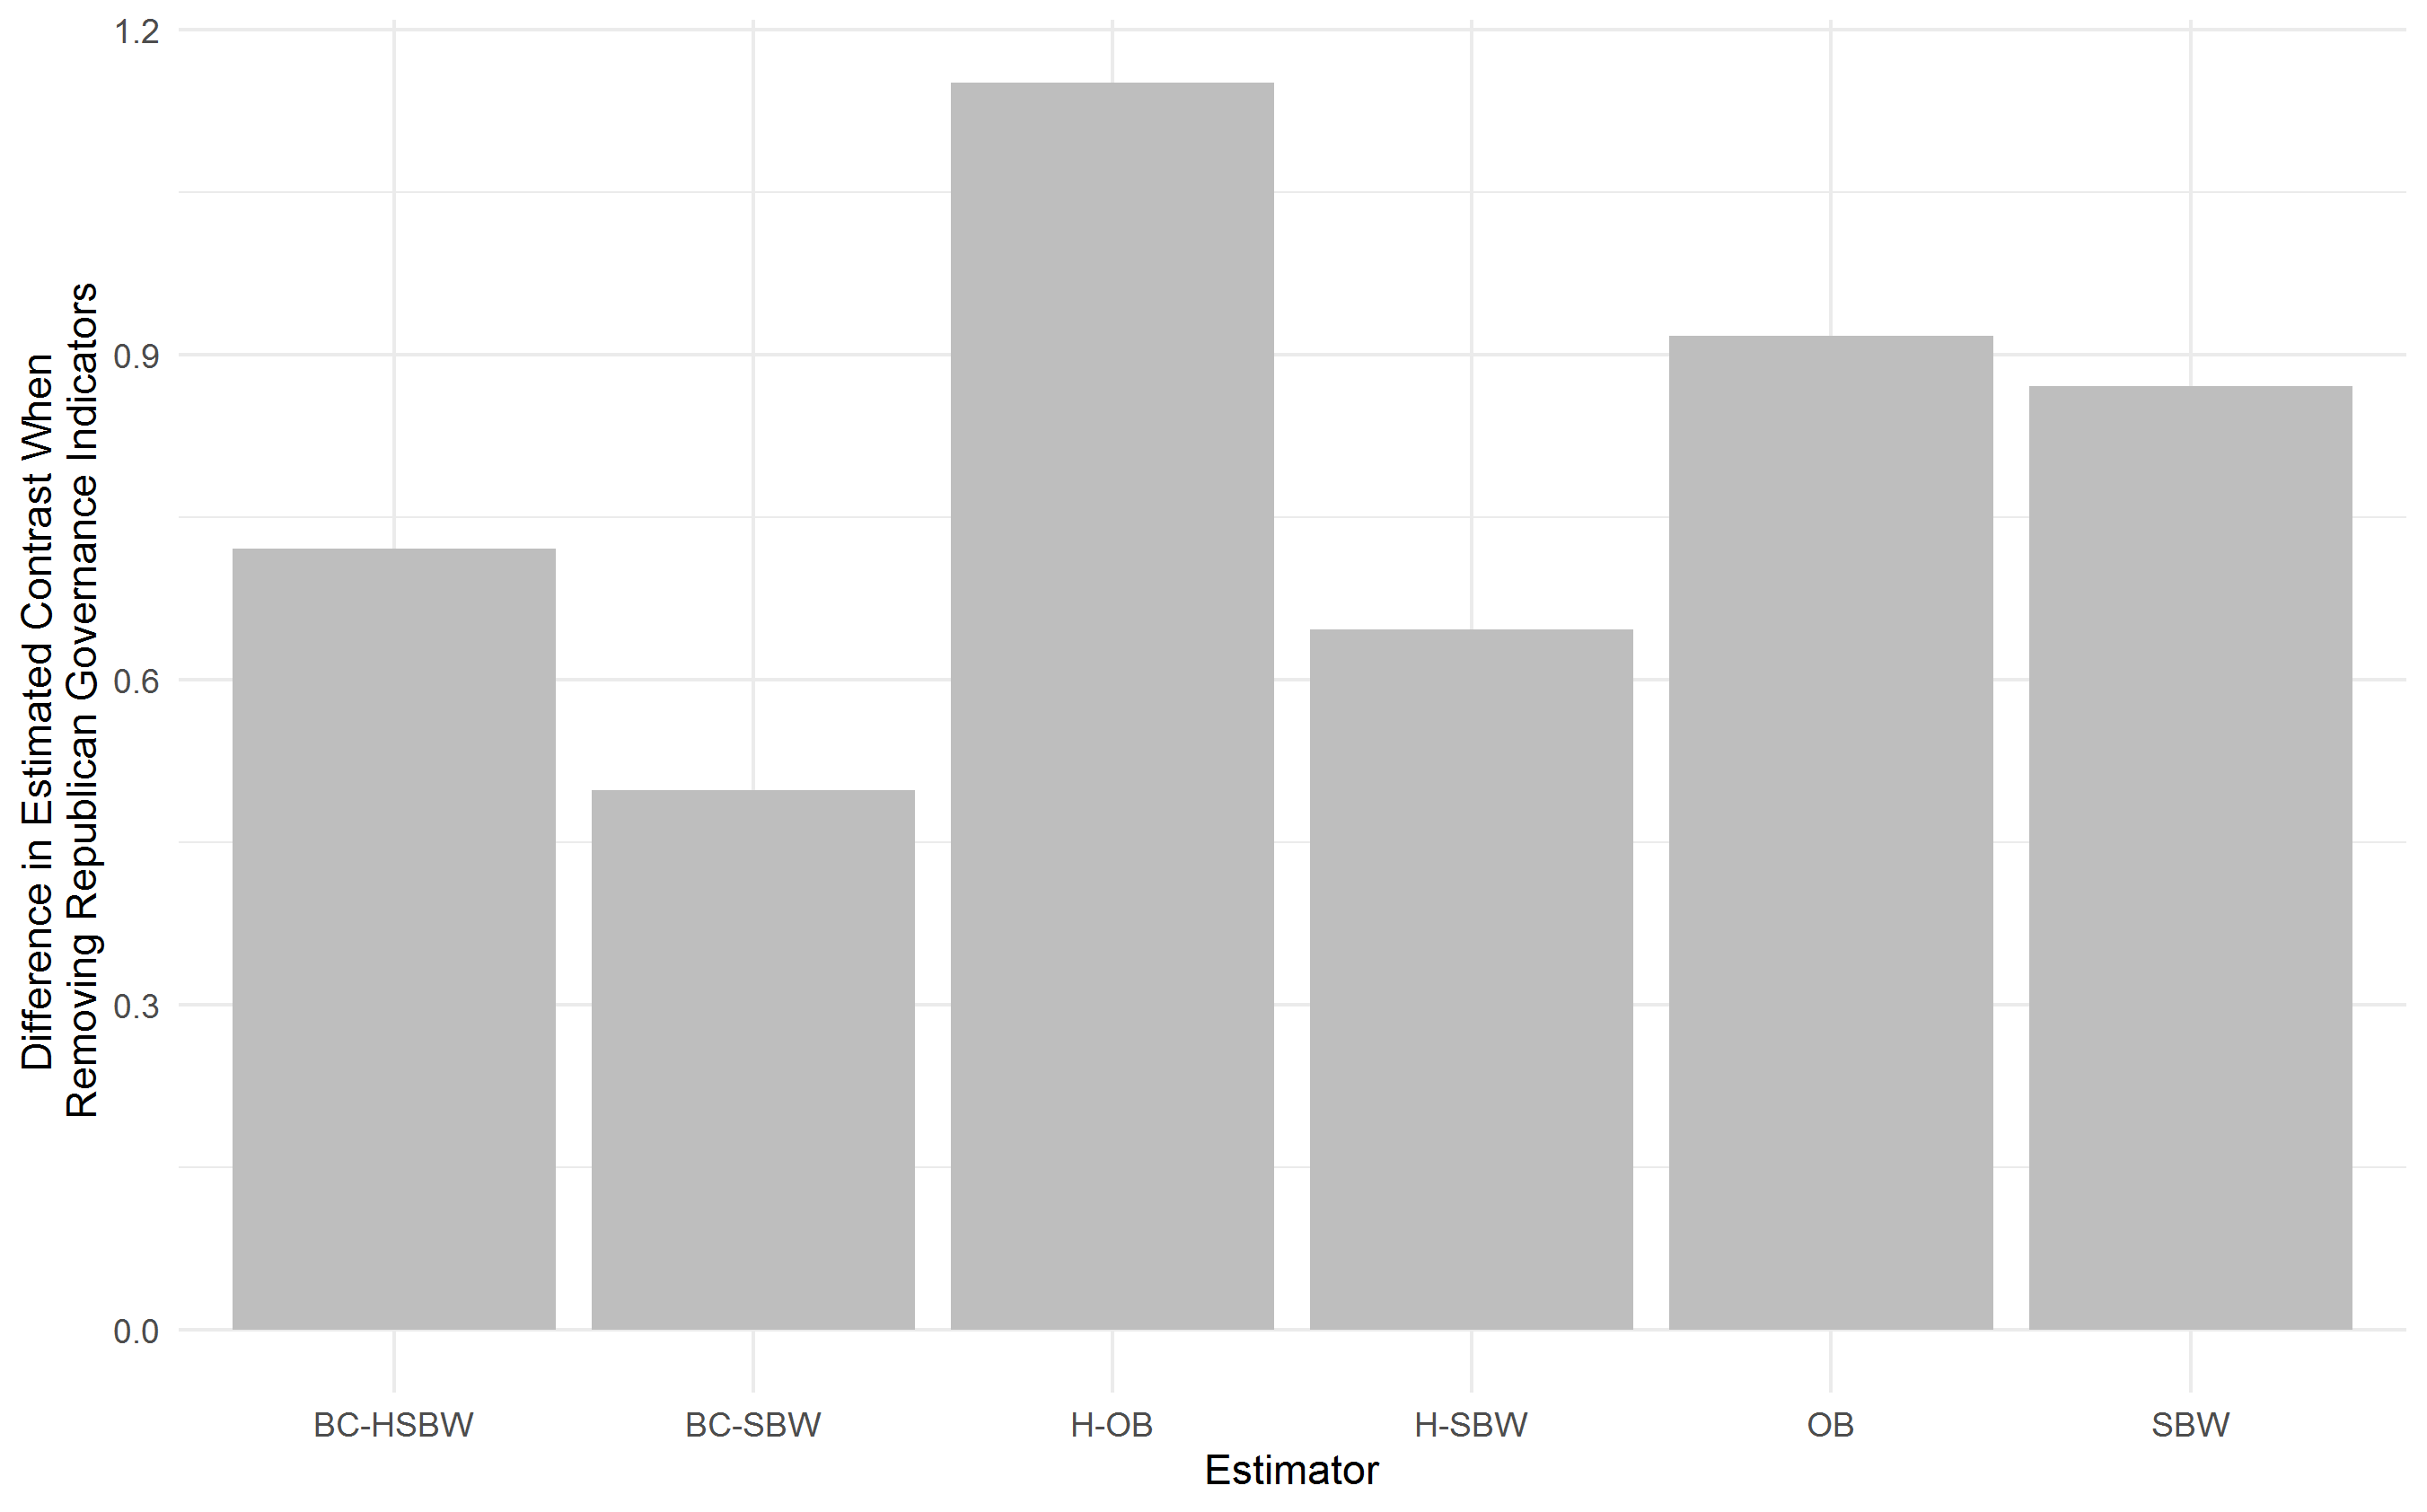
\includegraphics[scale=0.6]{01_Plots/repub-diff-c1.png}
    \caption{Removing Republican Governance Indicators}
    \label{repub}
\end{center}
\end{figure}

Finally, we analyze the sensitivity of our results to specific states. Given that the weighting procedure fits heavily to certain states, we are particularly interested in how the estimated causal effect might change when excluding these states.

\subsection{Sensitivity Analyses}

We now examine the sensitivity of our results to violations of two key causal assumptions: (1) no anticipatory treatment effects, and (2) positivity violations. To the first point, several states had partial limited expansions prior to 2014. Following \cite{frean2017premium}, we consider these states to be California, Connecticut, Minnesota, New Jersey, and Washington. We rerun our analyses excluding CPUMAs from all five of these states. We are unsure how we should expect this to affect our estimates: on the one hand, states that expanded early might have a smaller treatment effect after 2014 because they already enrolled newly eligible individuals. This would bias our previously estimated treatment effect upwards. On the other hand, if these states were also more motivated to enroll people in Medicaid, they might have larger post-expansion coverage gains, leading to a downwards bias. When removing these states, we estimate an effect of -1.35 (0.13, -2.83) using H-SBW weights and when we run the bias-corrected version we estimate -1.77 (-0.23, -3.32). Our leave-one-out covariate analysis shows similar associations to those in our primary analysis; however, we see a somewhat larger association between Republican governance indicators and our estimated contrast. In particular, we find that removing the Republican governance indicators increases our estimator by XX percentage points for HSBW, and by AA percentage point for HSBW. Figure XXX compares the association between the Republican governance indicators and the estimated treatment effect across four datasets: all treatment units included (our primary results), early expansion excluded, each with imputed and unadjusted covariates. This plot emphasizes that these associations hold regardless of whether or not we imputed the covariates or excluded the early expansion states.

We next consider positivity violations. To this point we have relied on either (1) leaving a potentially biased estimate from imbalanced weights, or (2) producing a more heavily model-dependent estimate that relies on extrapolation. Overall we found that the results didn't change substantially either way. Here We consider a third option: changing our target estimand. In particular, we consider the overlap average treatment effect (OATE), proposed by \cite{li2018balancing}. This is the treatment effect on the subset of the entire dataset where we have overlap. It is a data-dependent treatment effect, and is not the same as the treatment effect on the untreated; however, we believe that this effect will be more similar to the ETU than the ETT, since there were no Democratic controlled states that did not expand Medicaid. When generating overlap weights on our primary dataset we find support for this: across all covariates, the L2 distance from the overlap region to the treated region is XXX and to the untreated region is XXX. Figure XXX displays the sum of the weights within each state by treatment group. As predicted, we see that it is heavily represented by more conservative states, including Ohio, Arkansas, etc.

We find similar results to our primary analysis: within the overlap region we find an estimated treatment effect of -1.77 (-3.87 -0.06) when including all treatment states in our primary analysis, and of -1.89 (-3.14, -0.91) when excluding ``early expansion'' states (here we generate confidence intervals using the block bootstrap across 1000 iterations). We find that these estimates are not particularly sensitive to any one particular state. On the imputed dataset, removing Arkansas and Missouri resulted in the largest change in the estimated effect (moving it closer by 0.36 and 0.27 percentage points closer towards zero, respectively). We again find a negative association between the estimated contrast and the Republican governance indicators, which decrease the estimated effect size by 0.55 percentage points on the primary dataset and by 0.45 percentage points. Figure XXX displays the results when leaving out the Republican governance indicators for both the imputed and unadjusted datasets. Additional results are available in the Appendix.

\section{Discussion}

We estimate that had states that did not expand Medicaid in 2014 expanded their programs, they would have seen a VVV (QQQ, XXX) percentage point change in the adult uninsurance rate. Existing estimates place the ETT between -3 and -6 percentage points; these estimates vary depending on the targeted sub-population of interest, the data used, and the modeling approach (see, eg, \cite{courtemanche2017early}, \cite{kaestner2017effects}, \cite{frean2017premium}). This estimate is therefore closer to zero than these  papers, supporting our original hypothesis that the treatment effect on non-expansion states would be smaller in absolute magnitude. Moreover, we also find that we are likely to estimate treatment effects that are larger in absolute magnitude when allowing our comparison states to include states with more Democratic governance. This suggests that the differing political composition of the expansion versus the non-expansion states may explain these differences.

We also make several methodological contributions to the literature on balancing weights. First, we extending the synthetic controls literature to estimate the treatment effect on the untreated. The key challenge is that we are trying to predict treatment response rather than the outcome absent treatment. Unlike when estimating the treatment effect on the treated, we cannot use pre-treatment outcomes to conduct variable selection, run placebo tests, or train our model in some other way. This is a fundamentally more difficult problem that requires greater modeling assumptions. Second, we extend the Stable Balancing Weights objective for use with hierarchical data and measurement error. We modify the objective function to ensure that our weights more evenly disperse across states. We also exploit estimates of our region-level covariate estimates to account for bias induced by the measurement error by using a slight modification of standard regression calibration techniques.

Our study's approach also has bearing on estimating the ETT using a differences-in-differences to study the 2014 effects of Medicaid expansion. In particular, the consistent positive association between Republican governance and the estimated contrast between treatment and control states suggests that existing studies that fail to account for the interaction of treatment with measures of governance may incorrectly estimate the targeted treatment effects. We also find that there is likely insufficient overlap to account for these interactions without extrapolating from the data, and we show the ETU requires less extrapolation than the ETT with respect to these covariates. The primary estimand in the existing literature is instead the effect of treatment on the treated (ETT). While it may be tempting to extrapolate these findings to estimate the ETU (see, eg, \cite{miller2019medicaid}), this may lead to inaccurate inferences due to the heterogenous economic, demographic, and political characteristics between these groups of states.

Given that the effects of Medicaid expansion are primarily mediated through insuring the previously uninsured, we can assume that if the ETU were closer to zero than the ETT, then further downstream effects that grow monotonically with the number of insured would attenuate. For example, \cite{miller2019medicaid} use their estimate of the ETT to project that had all states expanded Medicaid in 2014, 15,600 deaths would have been avoided during their study's time-period. If we believe that the ETT were further away from zero than the ETU, we should expect that this number is an overestimate. Directly estimating the ETU in this context can therefore also help us better model interesting downstream effects mediated through increasing the number of insured individuals.

Our results come with the following caveats: (1) we rely on parametric assumptions about the outcome model to estimate our causal effect; (2) our identification assumes no unmeasured confounding, which is a relatively strong assumption; (3) spillovers across states might bias our estimates (and in general without redefining the causal estimand we cannot sign this bias); and (4) our variance estimation does not account for the variability induced by the measurement error in the covariates. 

We conclude by discussing the policy implications of these findings. First, we note that a reduction of adult uninsurance rates by -2.18 percentage points in represents approximately an eleven percent reduction in the pre-existing uninsurance rate for non-expansion states. This estimated treatment effect is closer to zero than corresponding estimates of the ETT (see, eg, \cite{courtemanche2017early}). We may therefore expect that downstream effects that move away from zero monotonically with the number of uninsured are also closer to zero than estimates of the ETT. For example, \cite{miller2019medicaid} estimate that if their set of non-expansion states had expanded Medicaid during their study period, they would have avoided 15,600 deaths. Because these estimates were based on projecting the ETT onto non-expansion states, assuming that avoided deaths increase monotonically with the number of uninsured, our results suggest that this figure may be an overestimate.

Second, we emphasize that the positive association we find between governance and the estimated treatment effect is only an association: this finding does not imply, for example, that states with Republican governments in general make Medicaid enrollment more difficult relative to Democratic states. However, this finding does not rule out this possibility either. Even if this causal story were true, then it is also a normative judgment whether this finding is a ``good'' or a ``bad'' result. To evaluate the policy implications, we compare this result against Congress's goal in implementing Medicaid expansion in the 2010 ACA, which was to increase health insurance coverage. Measured against this intent, this finding suggests that leaving states to implement individual enrollment schemes likely achieves sub-optimal results. Better federal policies should encourage states to adopt some form of automatic Medicaid enrollment, or to make Medicaid enrollment easier in some other way.

On the other hand, Republican governed states in 2014 were also more culturally conservative, and people may have been less likely to enroll in Medicaid due to social stigma and/or personal beliefs about the welfare state (\cite{sommers2012understanding}). If this remains true today, then Republican governments that are committed to expanding access to health care to low-income individuals may again wish to consider policies such as automatic enrollment to help mitigate these effects. Lastly, for Republican administrations who do not see coverage expansion as an important goal of Medicaid expansion, this finding may represent no policy problem at all.

\section{Conclusion}

This is the first study to directly estimate the foregone coverage expansions of Medicaid Expansion on states that did not expand Medicaid in 2014. We also contribute to the methodological literature on synthetic controls by clarifying the assumptions required to use longitudinal data to estimate the ETU rather than the ETT. We estimate that had states that did not expand Medicaid in 2014 done so, they would have seen a -2.18 (-1.31, -3.06) percentage point change in their uninsurance rate. This is substantially closer to zero than existing estimates of the ETT, which range between -3 and -6 percentage points. Regions from Ohio and Arkansa largely drive our initial estimates; however, we calculate similar estimates when excluding regions from any one particular expansion state. These estimates are also robust to sensitivity analyses examining potential violations of the assumptions of no anticipatory treatment effects and positivity violations. 

We also find evidence that Republican governance is associated with estimated effect sizes closer to zero. This association is also robust to the removal of each state, is consistent with existing estimates of the ETT that are also farther away from zero, and the finding that Medicaid take-up rates are lower in Republican-governed states prior to Medicaid expansion in 2014 (\cite{sommers2012understanding}). If the goal of Medicaid expansion is to increase access to insurance for low-income adults, this suggests that state and federal governments may wish to adopt policies that make Medicaid enrollment automatic, or at least easier.

\cleardoublepage
\bibliography{research.bib} 

\cleardoublepage

\section{Appendix}

\subsection{Appendix A: Proofs}

We prove Assertion 1, which is that the bias of the SBW estimator under measurement error is equivalent to the bias of the OLS estimator under the classical errors-in-variables model. 

We first outline the classical errors-in-variables setup. Consider the linear model $Y_i^1 = X_i^T\beta$ and assume we observe covariates $W_i \in \mathbb{R}^d$ which are a vector of mean-unbiased proxies for the true covariate $X_i$; ie $W_i = X_i + v_i$. Assume that $v_i \sim N(0, \Sigma_{UU})$ and $(X_i, W_i \mid A_i = a) \sim MVN((\mu_{a}, \mu_{a}), \Sigma)$, where 

$$
\Sigma = \begin{pmatrix} 
\Sigma_{XX} & \Sigma_{XX} \\ 
\Sigma_{XX} & \Sigma_{WW} 
\end{pmatrix}
$$ 

In a slight departure from the classical setup, we also consider the treatment indicator $A$, and for simplicity we assume that $\Sigma_{WW \mid A = 1} = \Sigma_{WW \mid A = 0} = \Sigma_{WW}$ and $\Sigma_{XX \mid A = 1} = \Sigma_{XX \mid A = 0} = \Sigma_{XX}$. This is not a necessary assumption, but rather a simplifying one for this proof (we do not assume this when estimating our models). Finally, because of the joint normality of $X_i$ and $W_i$, we also know that that $\mathbb{E}_W\{X_i \mid W_i, A_i = 1\} = \mu_1 + \kappa^T(W_i - \mu_1)$, where $\kappa = \Sigma_{WW}^{-1}\Sigma_{XX}$.\footnote{For simplicity, we omitted an error term in the model for $Y_i$; if we include this we also add the assumption that this error term is uncorrelated with the measurement error in $X_i$.} 

Recall that the bias of the OLS estimator of $\beta$ is $\beta - \hat{\beta} = \kappa^T\beta$. We can express our causal estimand as $\mu_1^T\beta$, and (accounting for the intercept), we see that the bias of this linear combination is $(\mu_0 - \mu_1)^T(I_d - \kappa)^T\beta$. We now consider the SBW estimator that sets $\delta = 0$ and show that this estimator has the same bias. The intuition for this result is as follows: weighting estimators estimate an implicit $\beta$ on a subset of the data where we have sufficient overlap. We can think of the implicit beta as the solution to some weighted-least squares problem. Because we assume that the outcome model holds on all of the data, WLS and OLS are estimating the same $\beta$; therefore, the bias that affects the least squares solution will have the same effect on the weighting estimator.  

More formally now, define the SBW estimator as:

$$
\arg\min_{\gamma \in \Gamma} \gamma_i^2
$$

$$
\Gamma := \{\gamma: W_1^T\gamma = W_0^T1, \gamma_i > 0, \gamma^T1 = 1\}
$$

\begin{align*}
    \mathbb{E}\{\hat{\psi}\} - \psi &= \sum_{i: A_i = 1}w_iY_i - \sum_{i: A_i = 0}Y_i^0 \\
    &= \mathbb{E}\{\beta^T(\sum_{i: A_i = 1} \gamma_i (X_i - v_i) - \sum_{i: A_i = 0} (X_i - v_i))\} \\
    &= \beta^T(\sum_{i: A_i = 1} \gamma_i\mathbb{E}\{v_i \mid W_i, A_i = 1\}) \\
    &= \beta^T(\sum_{i: A_i = 1} \gamma_i\mathbb{E}\{(W_i - X_i) \mid W_i, A_i = 1\} \\
    &= \beta^T(\sum_{i: A_i = 1} \gamma_iW_i - \sum_{i: A_i = 1} \gamma_i\mathbb{E}\{X_i \mid W_i, A_i = 1\})
\end{align*}

Substituting our expressions for the conditional distribution of $X_i \mid W_i, A_i = 1$, and taking expectations over $W_i$, we obtain:

\begin{align*}
    &= \beta^T(\mu_0 - \sum_{i: A_i = 1} \gamma_i(\mu_1 + \kappa^T(W_i - \mu_1)) \\
    &= \beta^T(\mu_0 - \mu_1) - \beta^T(\sum_{i: A_i = 1}(\gamma_iW_i - \mu_1))\kappa \\
    &= (\mu_0 - \mu_1)^T\beta - (\mu_0 - \mu_1)^T\kappa\beta \\
    &= (\mu_0 - \mu_1)^T(I_d - \kappa)^T\beta
\end{align*}

Adjusting for the bias induced by measurement error is a well studied topic. We use regression calibration techniques, which are discussed at length in the measurement error literature (see, eg, \cite{carroll2006measurement}). This allows us to adjust our covariates without using the outcomes, in the spirit of the design-based estimation strategy we use here. The consistency of our estimator follows from the results in the regression calibration literature. See CITE in particular, who consider the setting where we estimate the covariance matrices on auxillary data, and the $\Sigma_{WW}$ on the estimator. They also show the consistency of this estimator when we consider $X$ fixed and the model is misspecified. These results hold here since we are also assuming a linear and additive outcome model.

Proposition II. 

Let $X_{ij} \mid W_{ij} = \kappa^TW_{ij} + v_{ij}$, where $v_{ij} \sim N(0, \Sigma)$. Then: 

\begin{align*}
    \sum_{ij}w_{ij}Y_{ij} - \sum_{ij}Y_{ij} &= \sum_{ij}w_{ij}\kappa^TW_{ij}\beta + v_{ij} - \sum_{ij}X_{ij} \\
    &= \beta^T\sum_{ij}w_{ij}v_{ij}
\end{align*}

This term is mean-zero in expectation.

Proposition III.

We next argue that the variance of our estimator is dominated by the between group variance.

\begin{align*}
    \eta_{ij} = X_{ij}^T\beta + \epsilon_{ij} + c_j \\
    \implies Y_{ij} = X_i^T\beta + v_{ij} + \epsilon_{ij} + c_j \\
    \implies \mathbb{E}\{Y_{ij} \mid W_{ij}\} = \mathbb{E}\{X_{ij} \mid W_i\}^T\beta + v_{ij} + \epsilon_{ij} + c_j \\
    Var(Y_{ij} \mid W_{ij}) = \beta^TCov(X_{ij} \mid W_{ij})\beta + v_{ij}^2 + \epsilon_{ij}^2 + c_j^2 + 2\sum_{i\ne k}\rho_{ij} \\
    \implies Var(\sum_{ij}w_{ij}Y_{ij}) = \sum_{ij}w_{ij}^2() + \sum\sum_{i\ne k}w_{ij}w_{kj}\rho_{ij}
\end{align*}

Assume $\beta_j \le M$ and that the dimension of the covariates is $d$. Notice first that $Cov(X_{ij} \mid W_{ij})$ is a sample-average and therefore $\beta^TCov(X_{ij} \mid W_{ij})\beta = o(d^2/\sqrt{s_{ij}})$. The overall estimator is then $o(d^2/N_cs)$, assuming that these covariances are not correlated within block. We also have an $o(1/N_cs)$ term in the error equation since $Y_i$ is also measured with error; and, in general, we think of this term as small and not worth adjusting for (see, eg, CITE). Finally, we have the model error terms in the equation $\epsilon_{ij} + c_j$, again, the first term in the average $Y_i$ will be $o(1/\sqrt{N_c})$ while the second is $o(1/\sqrt{M_c})$. Asymptotically, the variance of this estimator is dominated by the number of states, rather than CPUMAs or the sampling variability as long as $d/M_c > d^2/N_cs$, or $N_cs > dM$. Since $min_{s} \approx N_c \approx 500$ and $d = 35$ and $M = 50$, this condition is clearly satisfied. Moreover, we see that for this application the order is much larger for the intergroup correlation. Therefore, we feel comfortable with simply running cluster-robust standard errors for this application.


We now prove the efficiency of our objective function assuming group-level dependencies in the model errors. Assume that we observe $i$ counties within $j$ states and again assume a linear and additive outcome model for $Y_{ij}^0$:

$$
Y_i^0 = X_i^T\beta + \epsilon_{ij} + c_j
$$

Assume that $\mathbb{E}(\epsilon_{ij}) = \mathbb{E}(c_j) = 0$ and that $\mathbb{E}(\epsilon_{ij}c_j) = 0$. In other words, we have some positive dependence within each region. We now consider the variance of any weighting estimator $\hat{\psi} = N_t^{-1}\sum_{ij}w_{ij}Y_{ij}$ such that $\sum_{ij} w_{ij} = N_t$:

\begin{align*}
    Var(N_t^{-1}\sum_{ij}w_{ij}Y_{ij} \mid X_{ij}) &= N_t^{-2}(\sum_{ij}w_{ij}^2Var(Y_{ij} \mid X_{ij}) + \sum_{j=1}^{M_t}\sum_{i=1}^{n_j}Cov(Y_{ij}, Y_{jk} \mid X_{ij}) \\
    &= N_t^{-2} (\sum_j w_{ij}^2(\epsilon_{ij}^2 + c_j^2) + \sum_{j=1}^{M_t}\sum_{i=1}^{n_j}w_{ij}w_{kj}c_j^2)
\end{align*}

Assuming that $\mathbb{E}(c_j^2) = \eta^2$ and $\mathbb{E}(\epsilon_{ij}^2) = \sigma^2$ for all $i, j$, and letting $\rho = \frac{\eta^2}{\eta^2 + \sigma^2}$ we then get that

\begin{align*}
    Var(\hat{\psi}) \propto \sum_{j=1}^{M_t} w_{ij}^2 + \sum_{j=1}^{M_t}\sum_{i=1}^{n_j}w_{ij}w_{kj}\rho
\end{align*}

Minimizing this objective function will then minimize the variance of this estimator. See Rubinstein (2021) (forthcoming) for more details on the performance of this estimator under different simulated settings.

We have not yet considered how the variance induced by the measurement error interacts with the variance induced by group-level dependencies. Our assumption in this paper is that the order of the variance of the group-level dependencies will dominate the other components, so we focus on reducing this source of variability in our estimates. Future work could consider optimizing for the interaction between these two sources of variability that affect our estimator considered in this paper.

\subection{Appendix B: Calibration Details}

We estimate the covariance matrix $\Sigma_{UU, ij}$ for sampling variability for each CPUMA's by estimating

$$
\hat{\Sigma}_{UU, ij} = \frac{4}{80}\sum_{b=1}^{80}(X_{ij}^B - \bar{X}_{ij})(X_{b, ij} - \bar{X}_{ij})^T
$$

Let $\hat{\Sigma}_{WW \mid A_j = 1} = \sum_{j: A_j = 1} (W_{ij} - \bar{W})(W_{ij} - \bar{W})^T$ be an estimator for $\Sigma_{WW \mid A = 1} = \mathbb{E}\{(W_{ij} - \mu_w)(W_{ij} - \mu_w)^T\}$. Notice that this estimator is calculated on the original dataset. We then estimate $\Sigma_{XX \mid A = 1} = \mathbb{E}\{(X_i - \bar{X})(X_i - \bar{X})^T \mid A_j = 1\}$ using:

$$
\hat{\Sigma}_{XX \mid A = 1} = \Sigma_WW - \sum_{ij: A_j = 1} \Sigma_{UU, ij}
$$

Define

$$
\hat{\kappa} = (\hat{\Sigma}_{WW})^{-1}(\hat{\Sigma_{XX}})
$$

We can think of this matrix as an estimate coefficient vector of a linear regression of the (unobserved) vector $X_{ij}$ on (observed) $W_{ij}$. We can impute $\hat{X}_{ij}$ as

$$
\hat{X}_{ij} = \bar{W} + \kappa^T(W_{ij} - \bar{W})
$$

This is the standard imputation suggested by CARROLL. However, in our setting we know that there is substantial heterogeneity in the measurement error: in particular, regions with large populations are estimated quite precisely, while others are estimated much less precisely. Even for a given CPUMA, some covariates are measured using three years of data, and others only one. From 2011 through 2013, STATISTICS on sample sizes!! As a result, using the conventional regression calibration approach will affect estimates that we know are precisely estimated and ones that we know aren't in a similar way. 

Our preferred estimators therefore use an alternative approach where we model $\Sigma_{UU, ij}$ as a function of the sample sizes used to estimate each covariate. In particular, let $s_{ij}$ be the d-dimensional vector of the sample sizes used to estimate each covariate value for a given CPUMA. Let $S_{ij} = \sqrt{s_{ij}}\sqrt{s_{ij}}^T$. We pool our initial estimates of the CPUMA-level covariance matrices ($\hat{\Sigma}_{UU, ij}$) to generate $\hat{\Sigma}_{UU}^m = N_t^{-1}\sum_{ij} S_{ij} \circ \Sigma_{UU, ij}$. We then estimate $\hat{\Sigma}_{UU, ij}^m = \Sigma_{UU}^m \oslash S_{ij}$. From this we estimate $\hat{\Sigma}^m_{XX} = \hat{\Sigma}_{WW} - N_t^{-1}\sum_{ij}\hat{\Sigma}^m_{UU, ij}$. Finaly, we calculate $\kappa_{ij} = (\hat{\Sigma}^m_{XX} + \hat{\Sigma}^m_{UU, ij})^{-1}\hat{\Sigma}^m_{XX}$. The benefit of using this estimator is that we account for unit-level heterogeneity in the measurement error. Moreover, we can do this while getting the full efficiency of using all of the units in the modeling. One cost of this procedure is that this aggregation models all differences as a function of the sample sizes, and averages over any potential heterogeneity due to heteroskedasticity (ie the measurement error covariance matrix changes depending on the true value of $X_{ij}$). We present the results using the conventional approach in Appendix E.

\subsection{Appendix B: Complete Balance Table}

\ref{fullbaltab} displays the unweighted means for the expansion and non-expansion states. 


\subsection{Appendix C: Additional Results}

\subsection{Appendix D: SBW Program Details}

We implement SBW using a modification of Noah Griefer's ``optweight'' package available in R. The modifications are available on ``github.com/mrubinst''. We use this program to generate weights that balance the means of the following covariates in the treated group to the control group within an error tolerance, $\delta$. Tables I and II below specify $\delta$ as a percentage point differences in the mean covariate between the control and treatment groups (we then convert this into absolute difference when using the program). 

When estimating the weights on different subsets of the data, $\delta^\star$ is not guaranteed to converge. We therefore modify the program so that if it does converge, it relaxes some of the constraints until the program converges. In particular, we iterated through the  following relaxations that continue until convergence:

EXPLAIN MODELS HERE


\end{document}






